%%%%%%%%%%%%%%%%%%%%%%%%%%%%%%%%%%%%%%%%%
% University/School Laboratory Report
% LaTeX Template
% Version 3.1 (25/3/14)
%
% This template has been downloaded from:
% http://www.LaTeXTemplates.com
%
% Original author:
% Linux and Unix Users Group at Virginia Tech Wiki 
% (https://vtluug.org/wiki/Example_LaTeX_chem_lab_report)
%
% License:
% CC BY-NC-SA 3.0 (http://creativecommons.org/licenses/by-nc-sa/3.0/)
%
%%%%%%%%%%%%%%%%%%%%%%%%%%%%%%%%%%%%%%%%%

%----------------------------------------------------------------------------------------
%	PACKAGES AND DOCUMENT CONFIGURATIONS
%----------------------------------------------------------------------------------------

\documentclass{article}
\usepackage[margin=1in, footskip=40pt]{geometry}
\usepackage{float}
\usepackage{multicol}
\usepackage{textcomp}
\usepackage{caption}
\usepackage{gensymb}
\usepackage{circuitikz}
\usepackage{glossaries}
\usepackage{siunitx} % Provides the \SI{}{} and \si{} command for typesetting SI units
\usepackage{graphicx} % Required for the inclusion of images
\setlength{\skip\footins}{1cm}

\usepackage{amsmath} % Required for some math elements 

%\setlength\parindent{0pt} % Removes all indentation from paragraphs

\renewcommand{\labelenumi}{\alph{enumi}.} % Make numbering in the enumerate environment by letter rather than number (e.g. section 6)
\usepackage{tabulary}
%\usepackage{times} % Uncomment to use the Times New Roman font

\usepackage{listings}
\usepackage{color}

\lstdefinelanguage{BetaAssembly}
{keywords={ADD,ADDC,AND,ANDC,MUL,MULC,OR,ORC,SHL,SHLC,SHR,SHRC,
SRA,SRAC,SUB,SUBC,XOR,XORC,CMPEQ,CMPEQC,DIV,DIVC,XNOR,XNORC,
CMPLE,CMPLEC,CMPLT,CMPLTC,BR,BT,BF,BNE,BEQ,JMP,LD,ST,LDR,MOVE,
CMOVE,HALT,PUSH,POP,ALLOCATE,DEALLOCATE,CALL,RTN,XRTN,LONG,
WORD,STORAGE,GETFRAME,PUTFRAME},%
sensitive=true,%
alsoletter={\$},%
comment=[l]{\|},%
string=[b]",%
string=[b]'%
}


\definecolor{dkgreen}{rgb}{0,0.6,0}
\definecolor{gray}{rgb}{0.5,0.5,0.5}
\definecolor{mauve}{rgb}{0.58,0,0.82}

\lstset{frame=tb,
  language=BetaAssembly,
  aboveskip=3mm,
  belowskip=3mm,
  showstringspaces=false,
  columns=flexible,
  basicstyle={\small\ttfamily},
  numbers=none,
  numberstyle=\tiny\color{gray},
  keywordstyle=\color{blue},
  commentstyle=\color{dkgreen},
  stringstyle=\color{mauve},
  breaklines=true,
  breakatwhitespace=true,
  tabsize=3
}

%----------------------------------------------------------------------------------------
%	GLOSSARY
%----------------------------------------------------------------------------------------
\makeglossaries
\newglossaryentry{Beta}
{
  name=Beta,
  description={A 32-bit processor designed in the MIT course 6.004. RISC architecture with a limited instruction set.}
}

\newglossaryentry{galvo}
{
  name=Galvo,
  description={Short for galvanometer.}
}

\newglossaryentry{laser beta}
{
  name=Laser Beta,
  description={A Beta to control the laser display.}
}

\newglossaryentry{physics Beta}
{
  name=Physics Beta,
  description={A Beta to control the physics and game behavior.}
}

\newglossaryentry{sprite}
{
  name=Sprite,
  description={an individual object to be displayed by the laser projector (for example, the left paddle).}
}


%----------------------------------------------------------------------------------------
%	DOCUMENT INFORMATION
%----------------------------------------------------------------------------------------
\title{\vspace{6cm}Laser Pinball \\ Final Report \\\vspace{1cm} MIT 6.111} % Title

\author{Weston Braun, Pauline Varley, and Jake Isenhart} % Author name

\date{December 10, 2014} % Date for the report\

\begin{document}

\maketitle % Insert the title, author and date
\vspace{8cm}
\begin{center}
\begin{tabular}{l r}
Professor: & Gim P. Hom \\
Term: & Fall 2014
\end{tabular}
\end{center}

\pagebreak

\tableofcontents

\pagebreak

%----------------------------------------------------------------------------------------
%	INTRODUCTION
%----------------------------------------------------------------------------------------

\section{Introduction} \label{intro}

For our final project, we wanted to create a pinball-like arcade game on an FPGA that would be displayed on a wall by an RGB laser projector. The system would allow the user to reconfigure the gameboard by recognizing colored objects on a wall; each color would correspond to a different game object, and the objects would appear in-game in the location in which they were placed on the wall. This project was motivated by a desire to use technology for enjoyment rather than academics; while discussing what we might want to build for our final project we found that, over the course of our MIT educations, we hadn't had much of an opportunity to just play around with tech in the way we do outside of class. We wanted a project that we could get excited about and a project that we could share with our peers without too much explanation—a laser-projected game is, undoubtedly, very cool and fits that criteria to a tee.

In our implementation of the proposed design we encountered a series of unexpected difficulties that prevented us from finishing all planned elements of the project. Interfacing with the camera module was particularly difficult (see sections \ref{cameraintro} and \ref{camerasuck}), and implementing a physics engine in Verilog so complex that we decided to scrap the initial architecture entirely and build the project on Beta processors that we implemented using Verilog (section \ref{mbeta}). These challenges will be discussed further in section \ref{implementation}.

We did, however, accomplish several exciting things: design and implementation of a "µBeta" processor; functional image recognition that can detect red, green, and blue objects; physics emulation written entirely in assembly; and a laser-projected gameboard with paddles that can be controlled with an NES controller.  These successes will be further discussed in sections \ref{modules} and \ref{implementation}.


%----------------------------------------------------------------------------------------
%	SUMMARY
%----------------------------------------------------------------------------------------
\section{Summary} \label{summary}

\begin{figure}[H]
\begin{center}
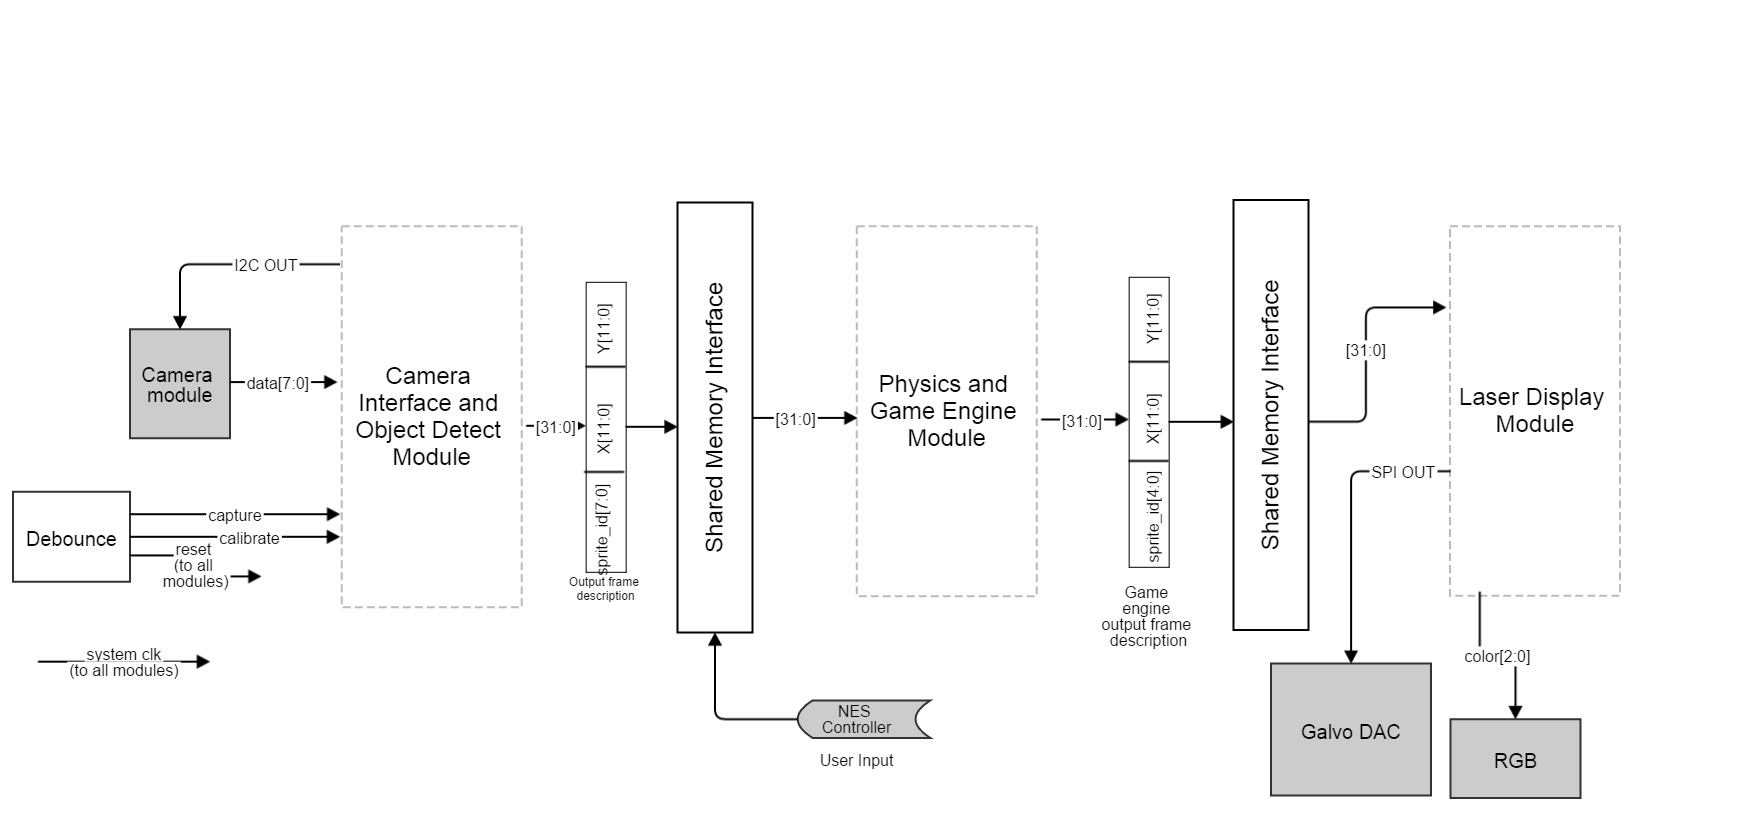
\includegraphics[width=\textwidth]{high_level_diagram} 
\caption{High-level system diagram. Each module will be explained in greater depth later in this report, and a full system diagram is included in the appendix.}
\end{center}
\end{figure}

Laser pinball was implemented as three discrete systems: a vision processing and object detect module, a physics and game engine, and a laser display controller.\footnote{Weston was responsible for the vision processing module; Jake and Pauline were primarily responsible for the physics engine and laser controller, respectively, but collaborated heavily on both. Weston also designed the external hardware interface and brought up the Beta processors.}  Though we originally planned on implementing the system entirely in Verilog, we realized about halfway through that the complexity of both the physics engine and the laser controller would be better suited to implementation on a microcontroller with a higher level of abstraction from the hardware. Since a Verilog implementation of the Beta processor already existed (to some degree—the bringup of the Beta will be discussed further in section SECTION NUMBER HERE), we decided to restructure both modules as assembly language code running on two separate Beta processors communicating via a shared memory interface. Despite this, the overall architecture of the system remained much the same.

The vision processing module takes input from an OV7670 camera, detects objects of three colors (one red, one green, and one blue), and outputs the corresponding sprite IDs and locations to the physics Beta processor over a shared memory interface. The physics engine detects collisions between the pinball and game objects and adjusts its position and velocity according to the game's internal physics. Finally, the laser display module plots sprites at arbitrary locations received from the physics module using a laser projector.

%----------------------------------------------------------------------------------------
%	MODULES
%----------------------------------------------------------------------------------------

\section{Modules} \label{modules}
\subsection{Vision Processing and Image Recognition} \label{vp}

\begin{figure}[H]
\begin{center}
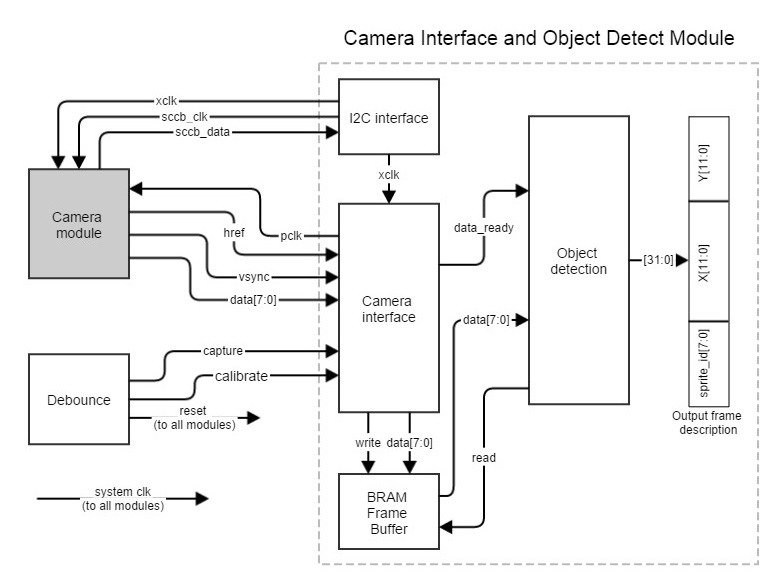
\includegraphics[width=0.75\textwidth]{camera} 
\caption{The camera interface module.}
\end{center}
\end{figure}

\subsubsection{The OV7670 Camera} \label{cameraintro}

The OV7670 camera was chosen because of its low cost and small size, allowing it to be mounted inside the laser projector case. The camera has an 8-bit output data bus, vertical (VSYNC) and horizontal (HREF) sync pins, and an output clock, and outputs 16-bit color over a 640x480 frame. The camera's output clock is internally generated by the camera from an input clock and is the same frequency as the input clock, but with different phasing. This required the crossing of clock domains within the FPGA. The camera outputs 8-bit wide sections of 16-bit wide pixels at twice the pixel clock frequency. An FSM was written in Verilog to synchronize the data capture of the camera with the start of the frame in order to capture a complete image. The frame starts on the falling edge of VSYNC and each line starts on the falling edge of HREF.

 Data captured from the camera was scaled down to 9-bit color and 240x240 pixels and stored in a dual port memory, which acted as a buffer to allow the crossing of clock domains. The down-sampling of color and resolution were due to constraints on the amount of BRAM within the FPGA and 9-bit resolution was used as the BRAM blocks have an input width of 9 bits: a byte plus a 9th bit storing a parity check value. We used this 9th bit to store additional color data. 
Unfortunately, the OV7670 camera has a quite complicated setup routine. The camera by default outputs YCrCb data instead of RGB. Additionally, the color balance is quite off to the point of red and green showing up reversed. The OV7670 camera contains a configuration interface called SCCB, which is essentially a royalty-free version of I2C and is I2C compatible. An open-source I2C core from the OpenCores project and licensed under the BSD license was used for I2C configuration. The core uses a Wishbone interface, which is an open source parallel bus standard. A Verilog FSM wrapper was written for the core to handle the Wishbone interface and an additional FSM was created to send configuration commands to the OV7670 camera from a ROM.

After image capture, the stored image was output to VGA using the Chrontel CH7301C DVI IC on the FPGA development board. This IC also required configuration over an I2C interface to be put in VGA pass-through mode. A version of the FSM used for camera configuration was reused to configure the Chrontel chip. 24-bit color is sent to the CH7301C through a 12-bit interface operating at twice the pixel clock by sending 12 bits at a time on each rising clock. A modified version of the VGA drive module from 6.111 lab 3 was taken to generate hsync and vsync signals for a 640x480 image at the faster pixel clock required by the CH7301C and to generate a pixel address to recall the stored image. A Verilog module was written to take 24-bit pixels and drive the 12-bit bus of the CH7301C. Image quality was poor for reasons which will be discussed further in section \ref{camerasuck}.

\begin{figure}[H]
\centering
\begin{minipage}{.5\textwidth}
  \captionsetup{width=0.8\textwidth}
  \centering
  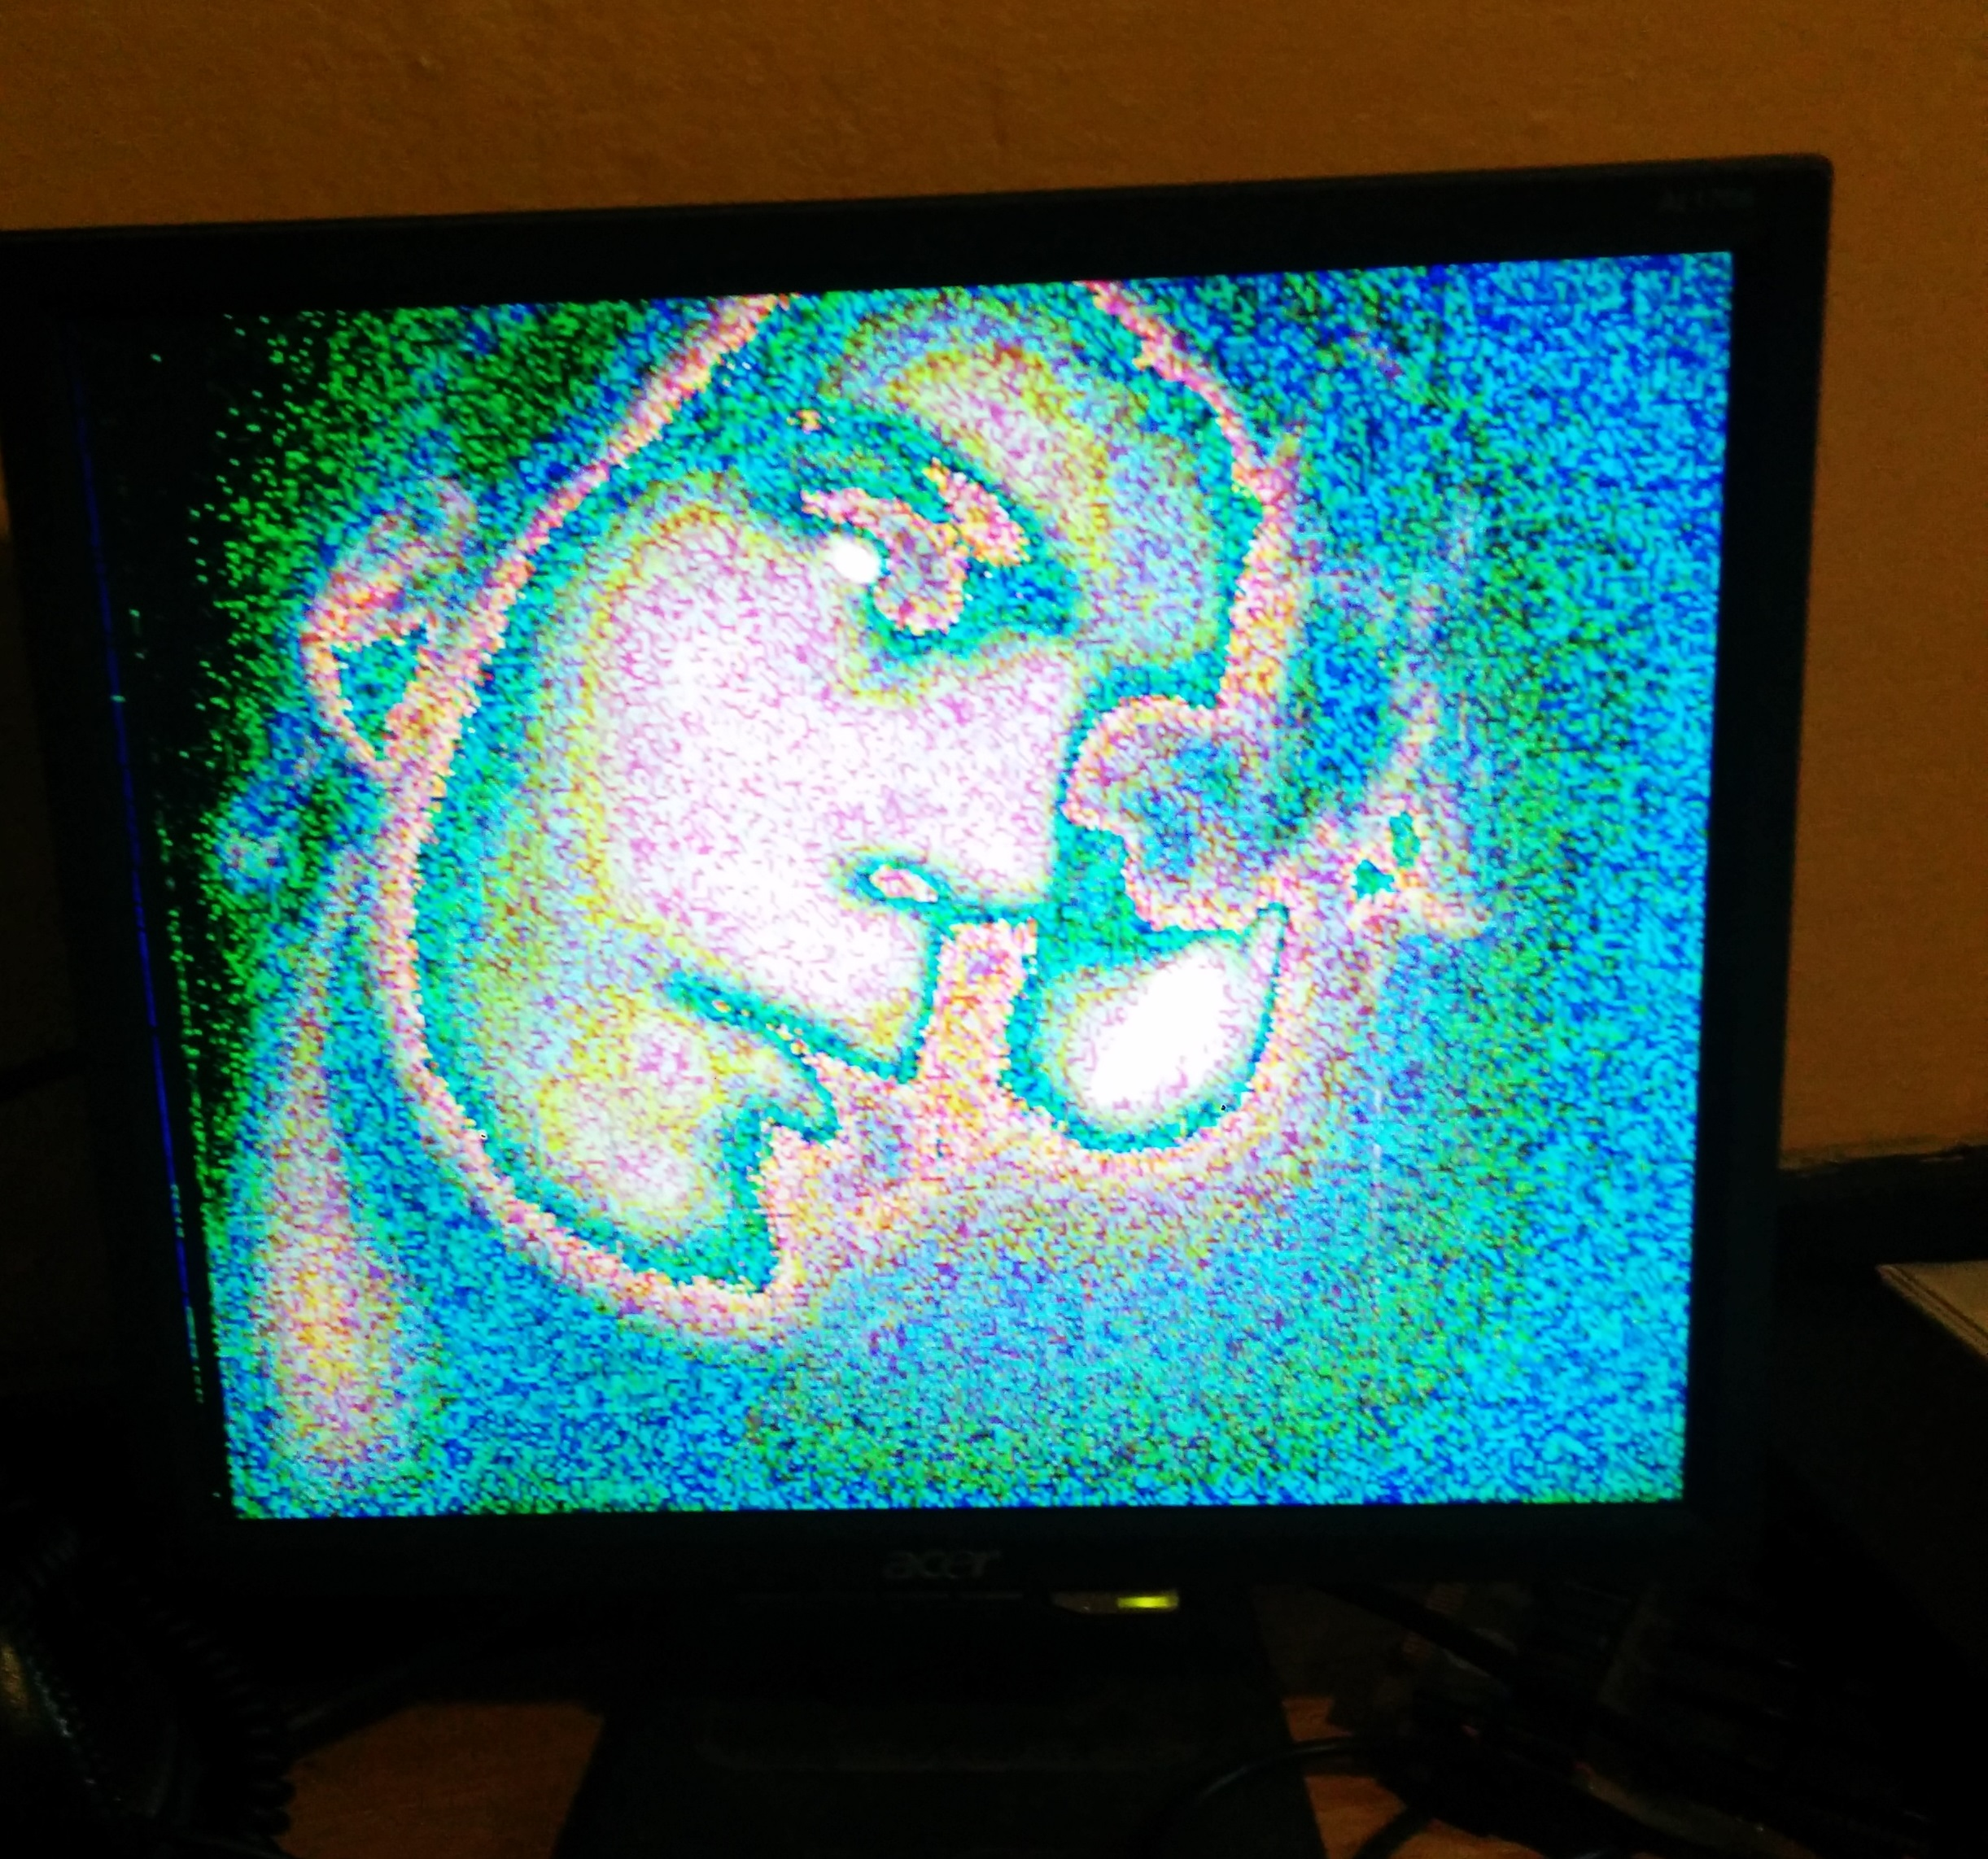
\includegraphics[height=2.5in]{weston}
  \caption{Camera output when an attempt was made to put it into RGB output mode.}
\end{minipage}%
\begin{minipage}{.5\textwidth}
  \captionsetup{width=0.8\textwidth}
  \centering
  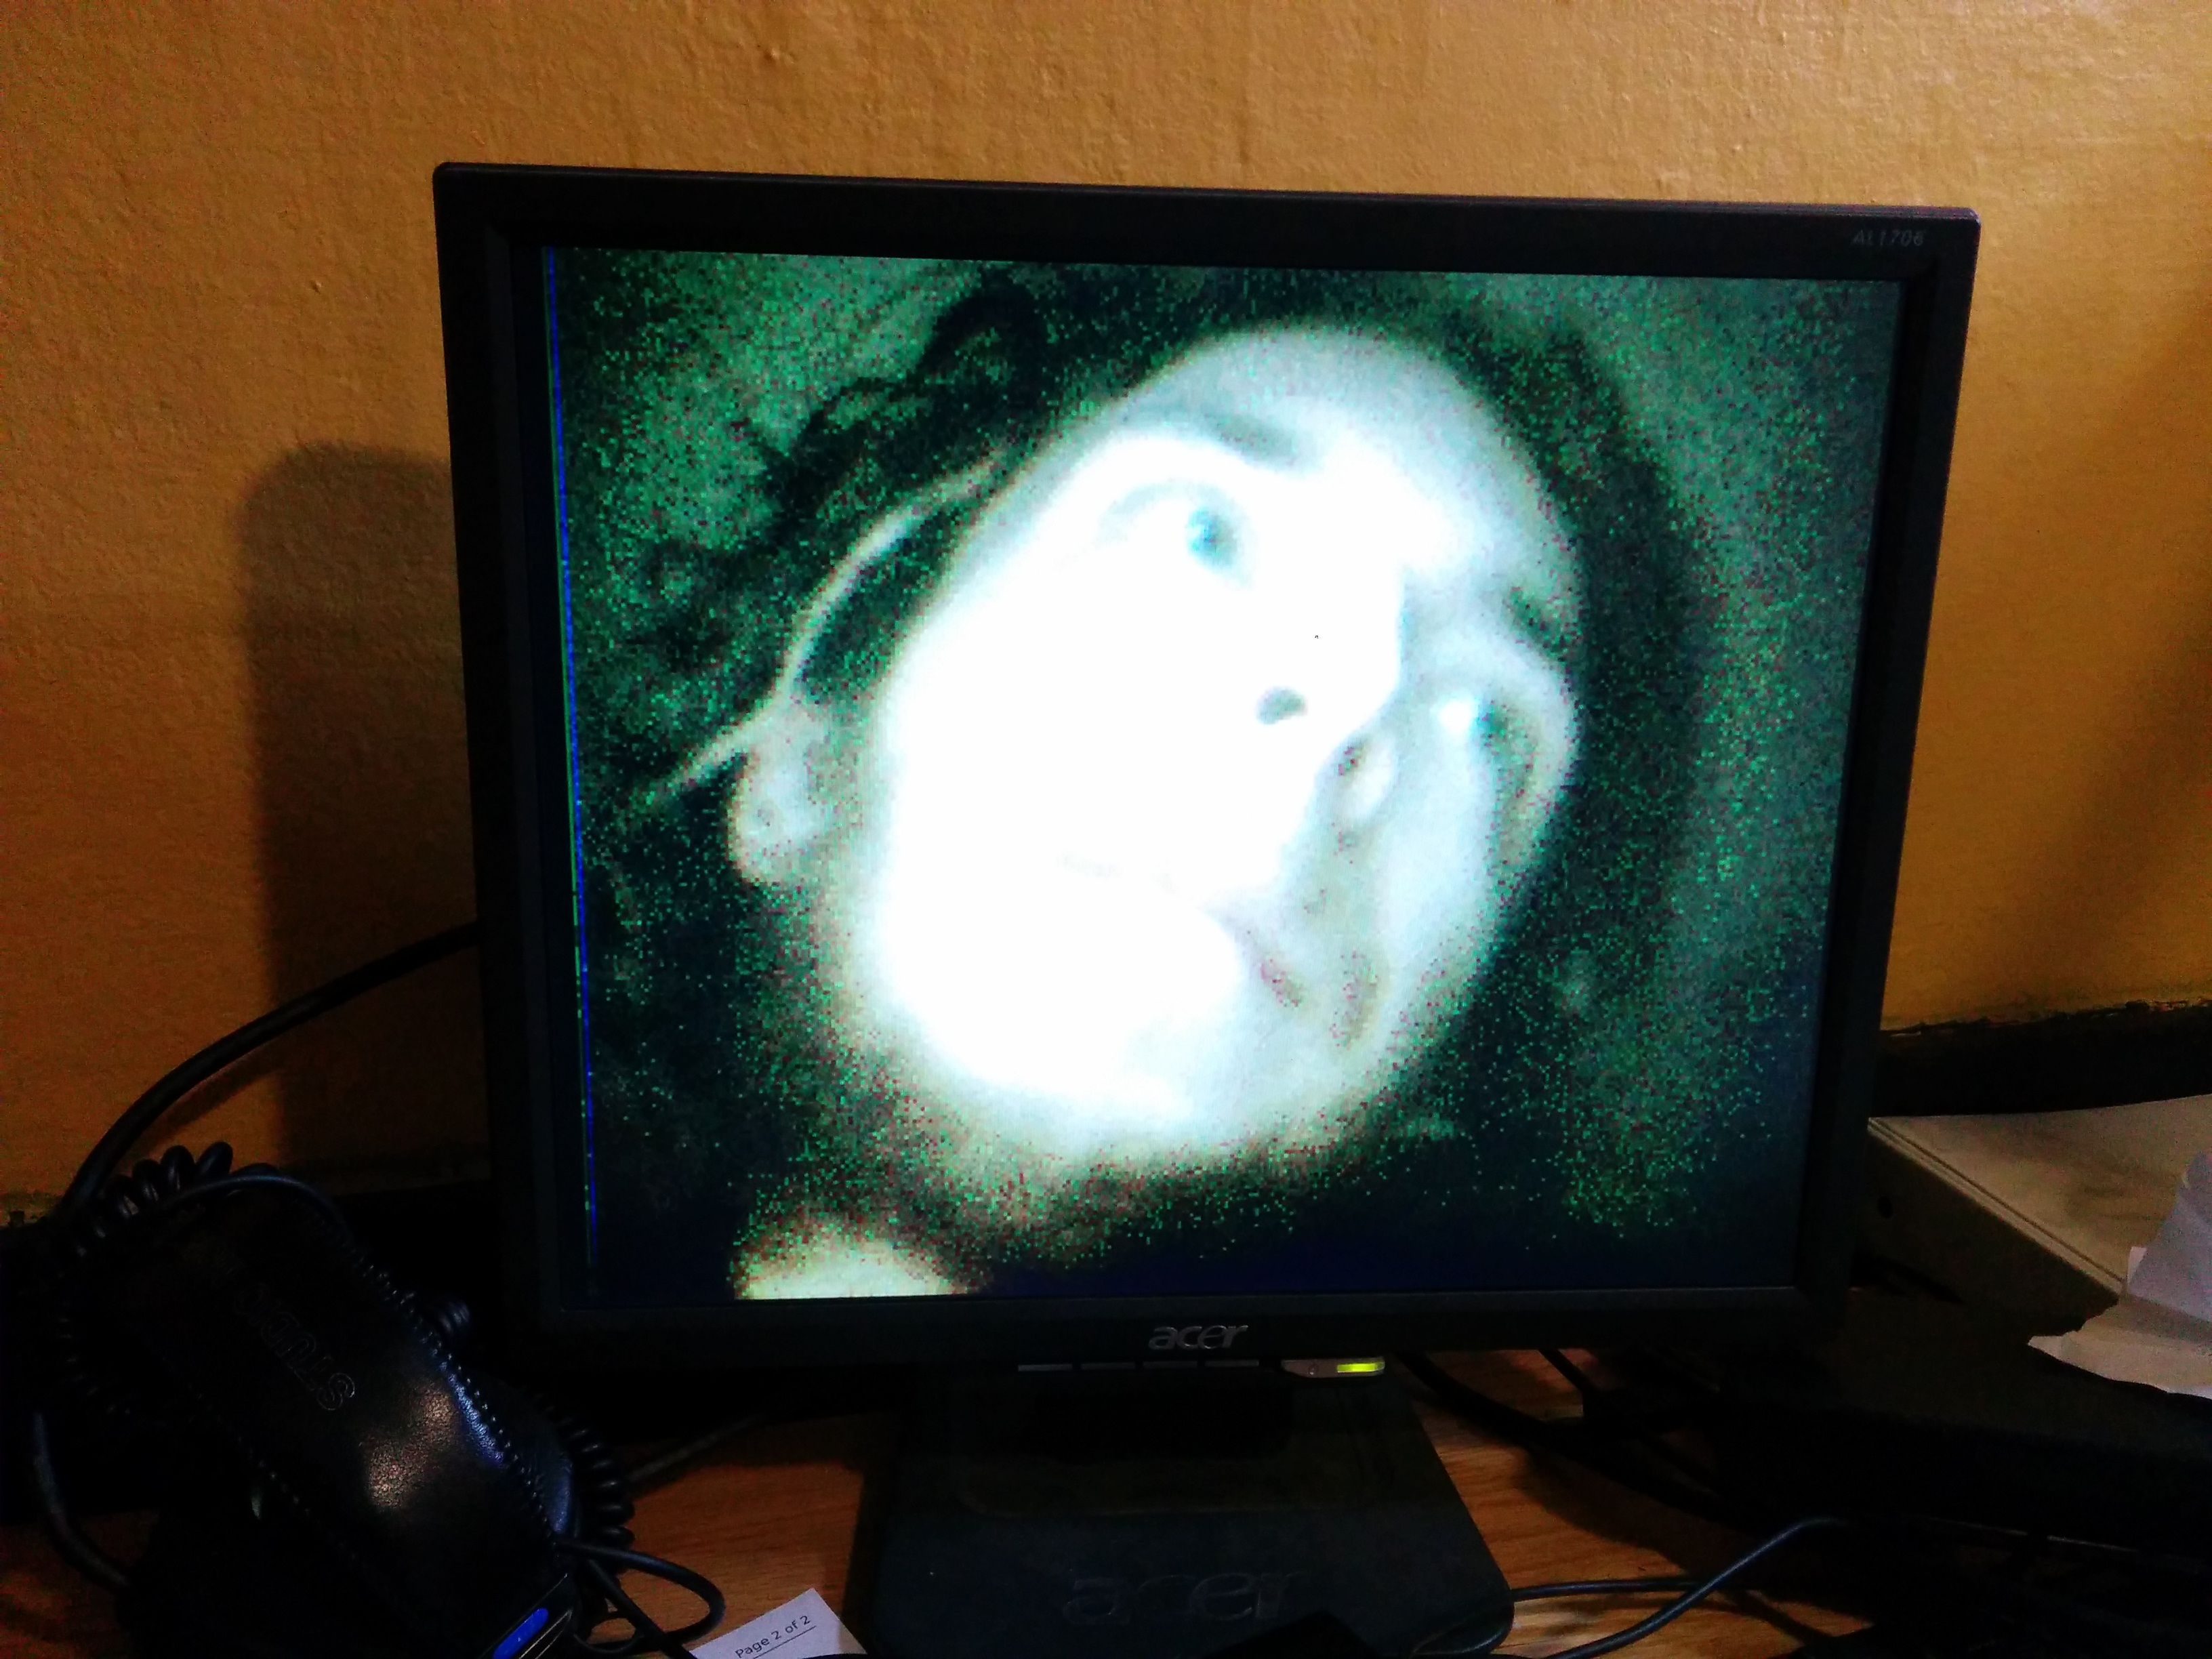
\includegraphics[height=2.5in]{peter}
  \caption{Camera output with the default settings.}
\end{minipage}
\end{figure}
	
\subsubsection{Image Recognition} \label{imagerec}

The goal of image recognition for the project was to recognize red, green, and blue game piece objects on a white background. As the game piece objects were to be small compared to the frame and were all primary colors, several simplifications could be made to the image processing process.

First, instead of calculating the mass of a single color, the image could be segmented into small sections, and a color classifier could be applied for each color that needed to be detected. The section of the image that had the the highest value for a given classifier was then detected as the center of a color block. 

The second simplification that could be made was in the classification of colors. Traditionally, the image is converted to the HSV color-space for classification. However, this process is computationally complex as it is not a linear mapping and requires the use of division, which is difficult to implement on an FPGA. Due to the low color resolution of the stored image and the need to only detect primary colors, a classifier was created that would directly translate an RGB color value into a set of color classifiers for red, green, and blue. This classifier would also have to reject mixtures of colors, such as white.
The classifier that was decided on for image recognition for each primary color was the value of the desired color minus the value of one of the other colors, multiplied by its value minus the other color. For red, this classifier would be $(red-green)\cdot(red-blue)$. This classifier worked well in distinguishing the colored game objects on a white wall. For processing, the image was split into 3600 squares of 16 pixels each. The 16 pixels in each block were averaged to remove noise and then run through the classifier. The three blocks that had the highest classifier values for red, green, and blue respectively were decided to be the coordinates of the detected objects. 

Image processing was implemented using a Verilog FSM that was triggered by a button on the FPGA board. Data was acquired from the read port of the dual port ram that the camera data was stored in, allowing the user to press a button to see live video from the camera, release the button to capture the frame, and then press a second button to analyze that particular frame. Once the frame was analyzed, a sprite was overlaid onto the stored image at the location of three detected color objects so that the user could confirm that the correct objects were recognized.

 Additionally, the location of each object was written into the memory space of the physics engine beta through the shared memory interface along with a done flag. 
 
\subsection{Physics and Game Engine} \label{physics}

\begin{figure}[H]
\begin{center}
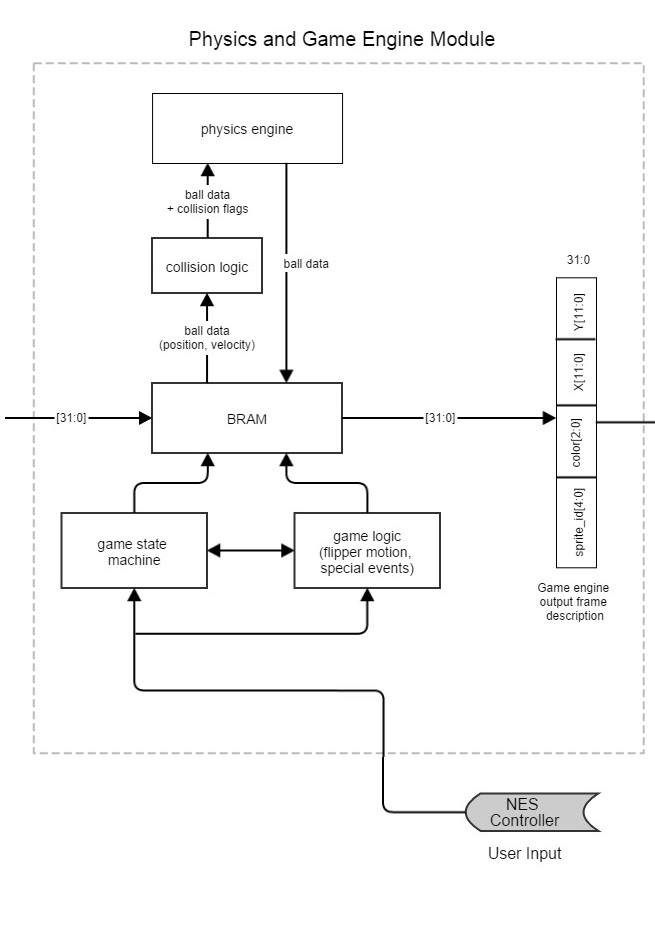
\includegraphics[width=0.5\textwidth]{physics} 
\caption{The physics and game engine module.}
\end{center}
\end{figure}

Initially, it was our intention to implement the entirety of the project in Verilog. Unfortunately, we had incorrectly assumed that the game logic would be almost an afterthought---how hard could it be to decide whether or not two objects are touching each other? Some cursory research on the subject of game engines informed us that it is, in fact, a very high-
level mathematical problem.

Unlike in the game of pong we put together in lab, we didn't have the luxury of calculating our collisions using fixed logic. Our plan was to have a game board which could be reconfigured without writing and compiling a new Verilog module. It became apparent in very short order that this wasn't going to be possible with fixed logic. In addition, we hoped to make our physics simulation more complex than that of the pong game; we wanted friction, gravity, and collisions with differing elasticities. In the pong game, whenever our ball hit an object, it was simple to calculate the resulting trajectory and velocity of the ball, because all of the collisions were perfectly elastic and took place with a surface perfectly aligned on either the x or y axis. In these simple cases, negating either the x or y velocity is enough to simulate a realistic collision. Collision detection with angled surfaces (like the triangular bumpers of our gameboard) requires vector math which would be prohibitively complicated to implement as a state machine. In addition, we wanted to have a variable number of game objects---the more we discussed what we needed in order to properly build our dream pinball game, the more we realized we were essentially describing a processor. 

With the realization that we wanted to be able to define parts of our project purely in software, we decided to look into the Verilog implementations of the 6.004 Beta core available on past versions of the 6.111 website. The Beta fit our specifications well. Its 32-bit architecture was adequate for doing complex math in the physics module, as well as precisely controlling the laser galvos in the projection module. In addition, it was free, and all of us had experience writing assembly code for it from 6.004. We also considered using other free cores like Xilinx PicoBlaze, but were discouraged by its 8-bit architecture, which would not afford us the precision to do accurate physics modeling, or even make full use of the 12-bit DACs we used to drive the laser galvos. The Beta architecture used for the project will be discussed in more detail in section \ref{mbeta}.


\subsubsection{The SNES Controller}
Though we had originally wanted to use accelerometers to control the pinball game's paddles, we instead decided to use an SNES controller because it was far simpler to read. We simply mapped its buttons to one of the Beta's memory-mapped input ports and were able to read digital values directly from the controller.

\subsection{Laser Controller} \label{laser}

\begin{figure}[H]
\begin{center}
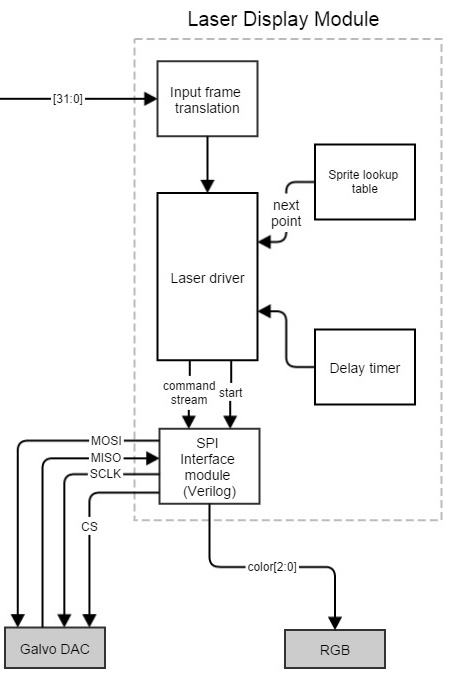
\includegraphics[width=0.5\textwidth]{laser}
\caption{The block diagram for the laser display module. Unless noted, all blocks were designed in Beta assembly language.}
\end{center}
\end{figure}

The laser display module was implemented primarily on a Beta processor, with the exception of the SPI interface module, which was implemented in Verilog as a simple state machine. The SPI module was then treated as a memory-mapped I/O device accessible by the laser Beta. Each frame, the laser Beta received form the physics Beta a series of one-word (32-bit) sprite descriptions detailing the ID of the sprite to be drawn, its color, and its x and y location within the frame.\footnote{Location was defined as the point in the upper left corner of the sprite, and sprites were drawn clockwise from this point.} A frame was known to be over if a null sprite ID was received; the physics and laser Betas could then easily coordinate frames by jumping back to the beginning of the shared memory space at the end of each frame, so first sprite in a frame was always stored at and read from shared memory location zero.

	For each sprite received, the laser controller first registered each part of the input word (sprite ID, color, x location, and y location) into separate registers. Sprite ID was then translated into an offset into the laser Beta's local sprite lookup table, a portion of which is shown below:

\begin{figure}[H]
\begin{center}
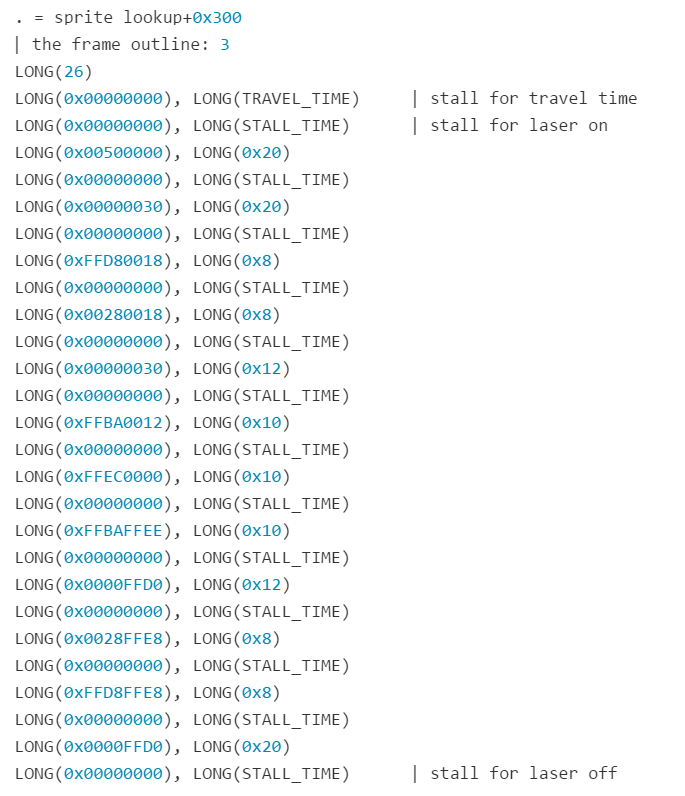
\includegraphics[width=0.75\textwidth]{sprite_lookup_laser}
\caption{The frame outline entry from the laser Beta's sprite lookup table.}
\end{center}
\end{figure}

Each sprite was broken up into line segments, and each line segment was broken up into sub-segments in order to not overdrive the galvos (which could only be driven a small distance at a time). The first item of each sprite (here "LONG(26)") is the number of line segments in that sprite. This was used as a countdown so the laser Beta knew when it had reached the end of the sprite. The numbers in the left column describe x (most significant two bytes) and y (least significant two bytes) offsets, and the numbers in the right column are the number of times the corresponding offset is repeated. These offsets describe the length and direction of each sub-segment.

 To draw the sprite, each offset in the table was split into its x and y components, sign-extended, and added to the initial x and y location received from the physics Beta; the initial location, which was registered, was then overwritten to store the current location. This new x-y point was then written to the galvos via the SPI module. A timer was set at 20kHz and the program delayed sending a new value to the galvos until the timer flag went high; during this period of time, the laser Beta polled two reserved shared memory locations for flipper trigger information, overwriting its stored paddle offsets in the sprite tables with new ones that appeared in the shared memory location. This allowed for the paddles to be updated to either their "up" or "down" positions every frame. This process was repeated with the same offset the specified number of times (drawing each sub-segment one at a time) until the end of the segment was reached; the next set of offsets was then loaded and the entire process was repeated until the segment counter ran out and the end of the sprite was reached. The process then began again with the next sprite.
 
Null offsets were inserted into the sprite table at the beginning and end to account for laser travel and power toggle time; null offsets were also added at sharp corners to counter the effects of the galvos' inertia.

\subsubsection{Galvanometers and DACs} \label{galvos}

The external hardware for the laser display—the DAC used to control the galvanometers, the laser, and the galvanometers themselves—were treated as memory-mapped peripherals and controlled simply by writing to and reading from the corresponding location in memory. Generating a coherent display on a laser projector, however, has a fair share of problems inherent to the hardware that must be solved. The two main problems were issues of inertia: the galvanometers are extremely slow compared to the 50MHz clock of the Beta, and driving them any faster than about 20kHz could break them; similarly, the laser has a not-insignificant power on and off time. These are some of the problems with commercial laser projection systems, as well: the inertia of the galvos tends to round out sharp corners, and the designer has to be careful of laser power during travels between sprites. These issues were accounted for in the sprite drawing process described above with the addition of "null offsets": the effects of these offsets can be clearly seen in the images below.

\begin{figure}[H]
\centering
\begin{minipage}{.5\textwidth}
  \captionsetup{width=0.8\textwidth}
  \centering
  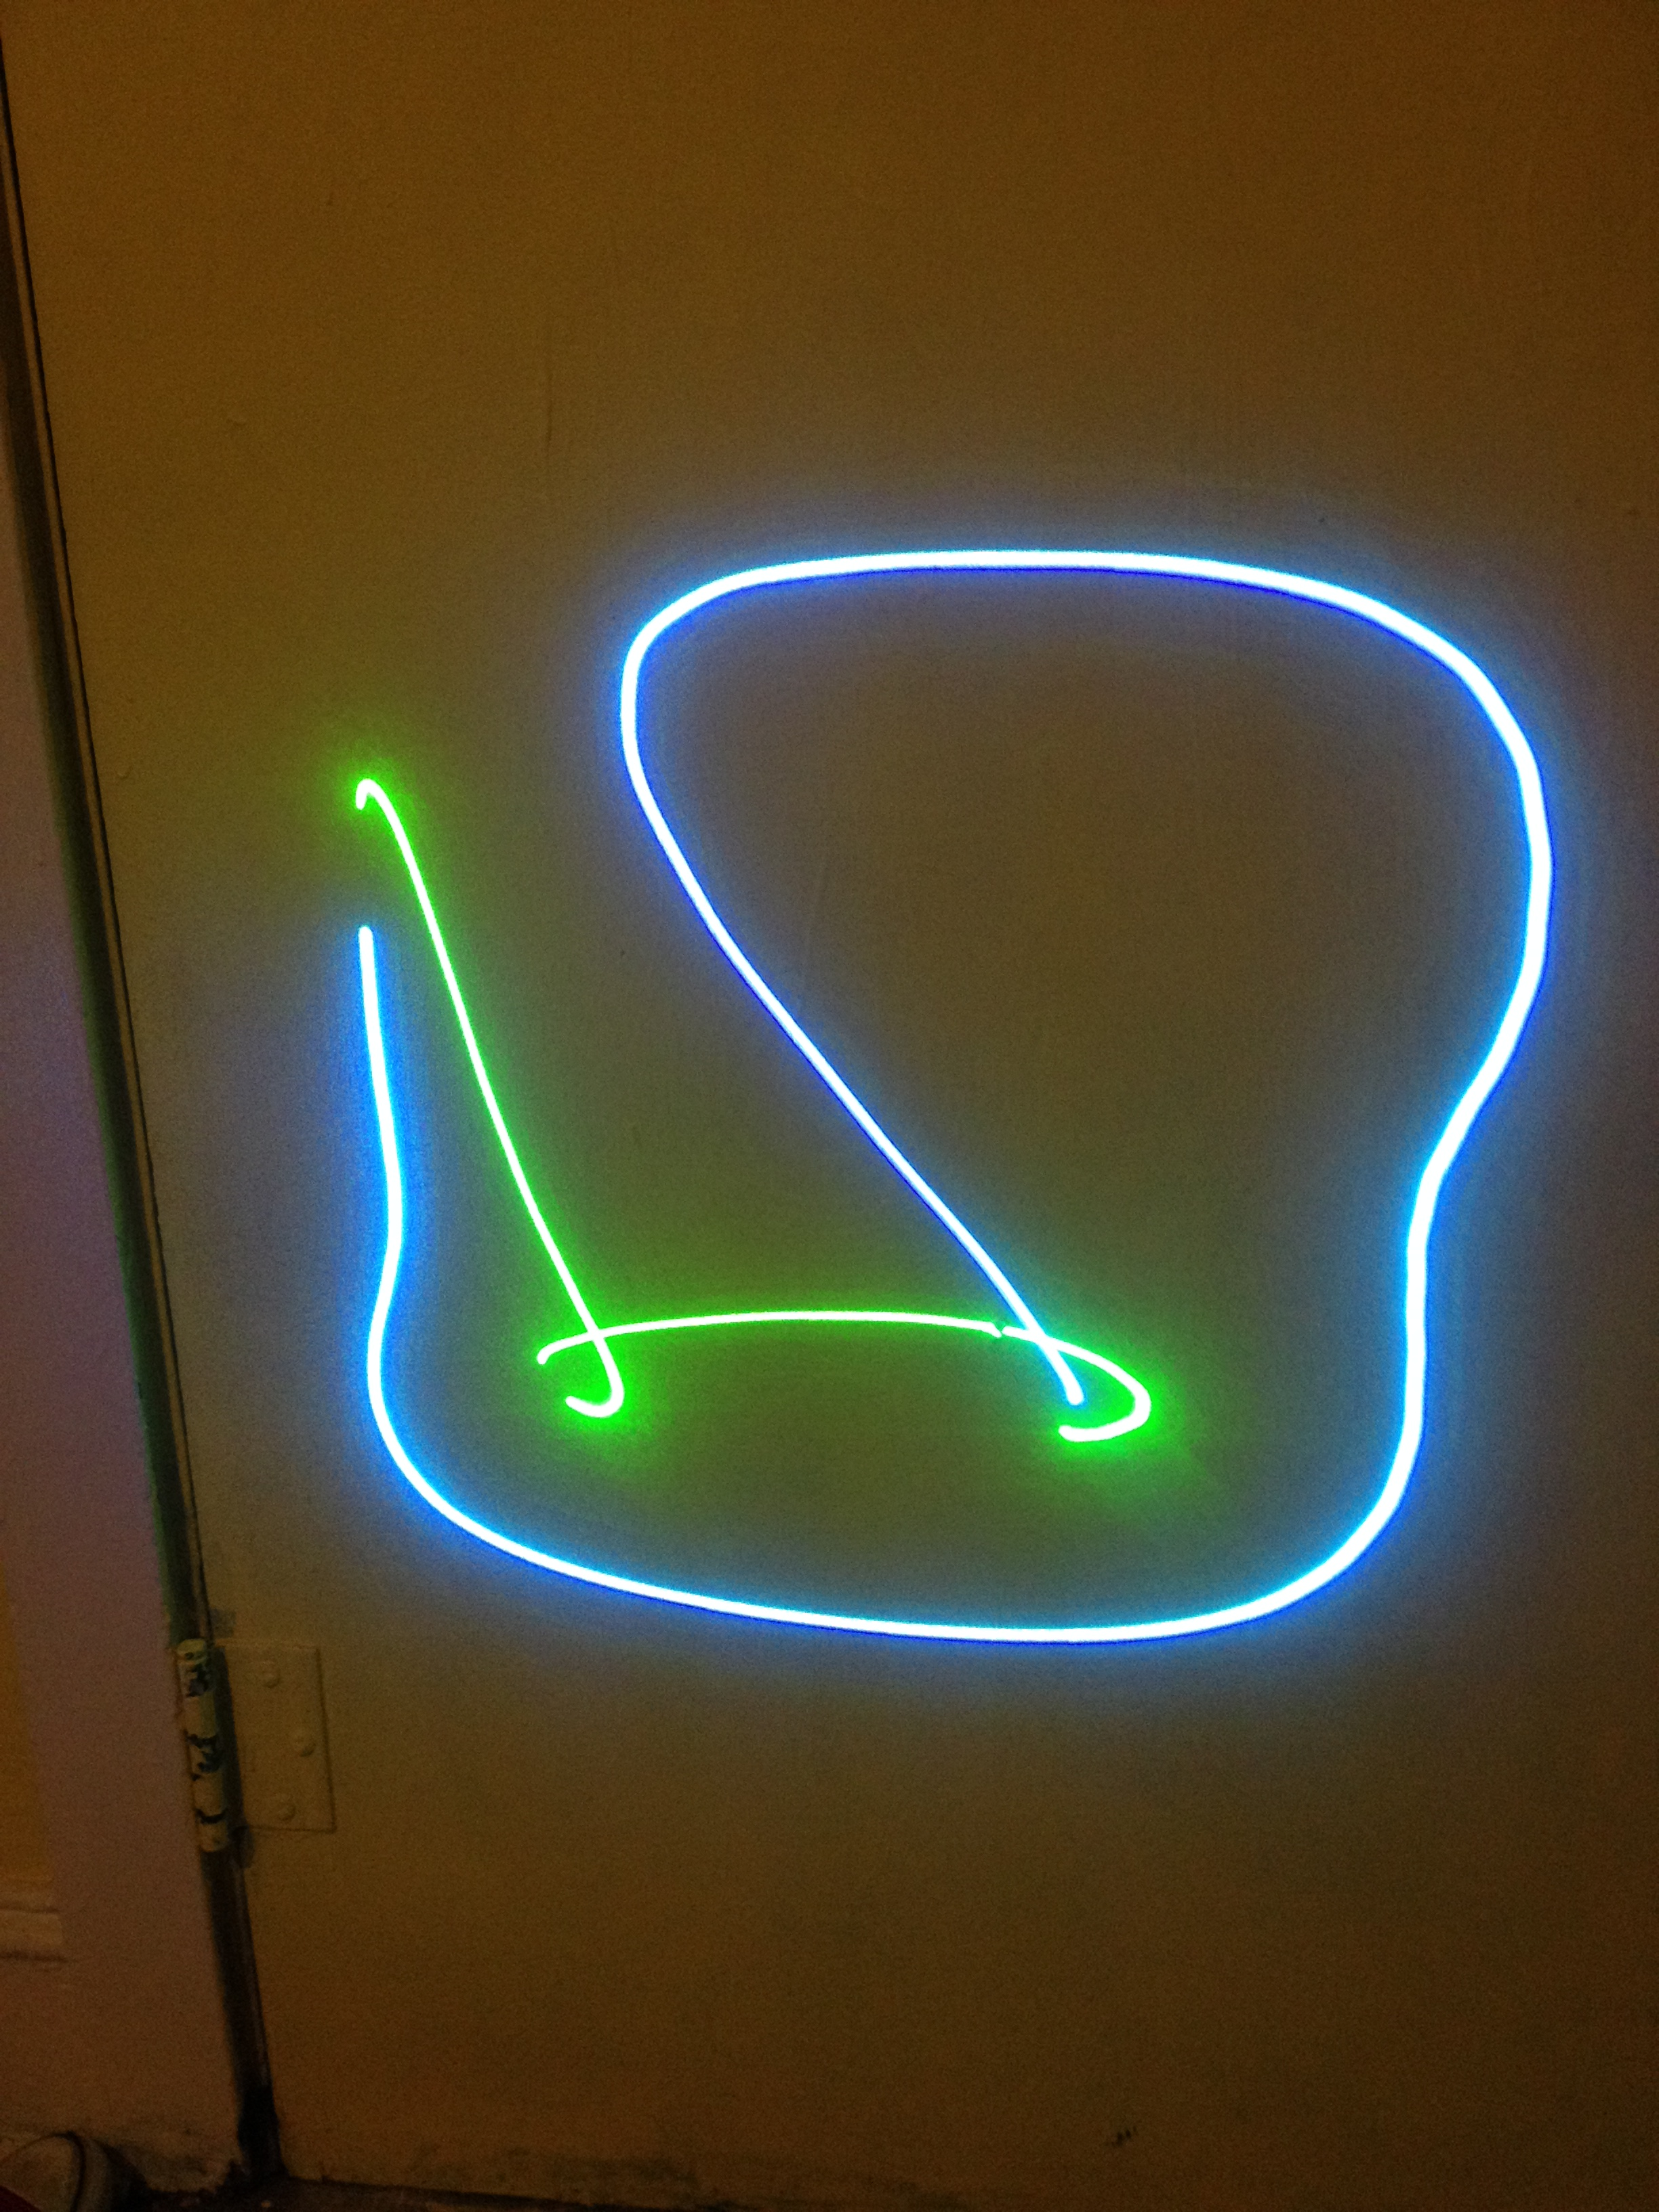
\includegraphics[width=.6\linewidth]{laser_loopy}
  \caption{The display without corner stalls or stalls for laser power.}
  \label{fig:loopy}
\end{minipage}%
\begin{minipage}{.5\textwidth}
  \captionsetup{width=0.8\textwidth}
  \centering
  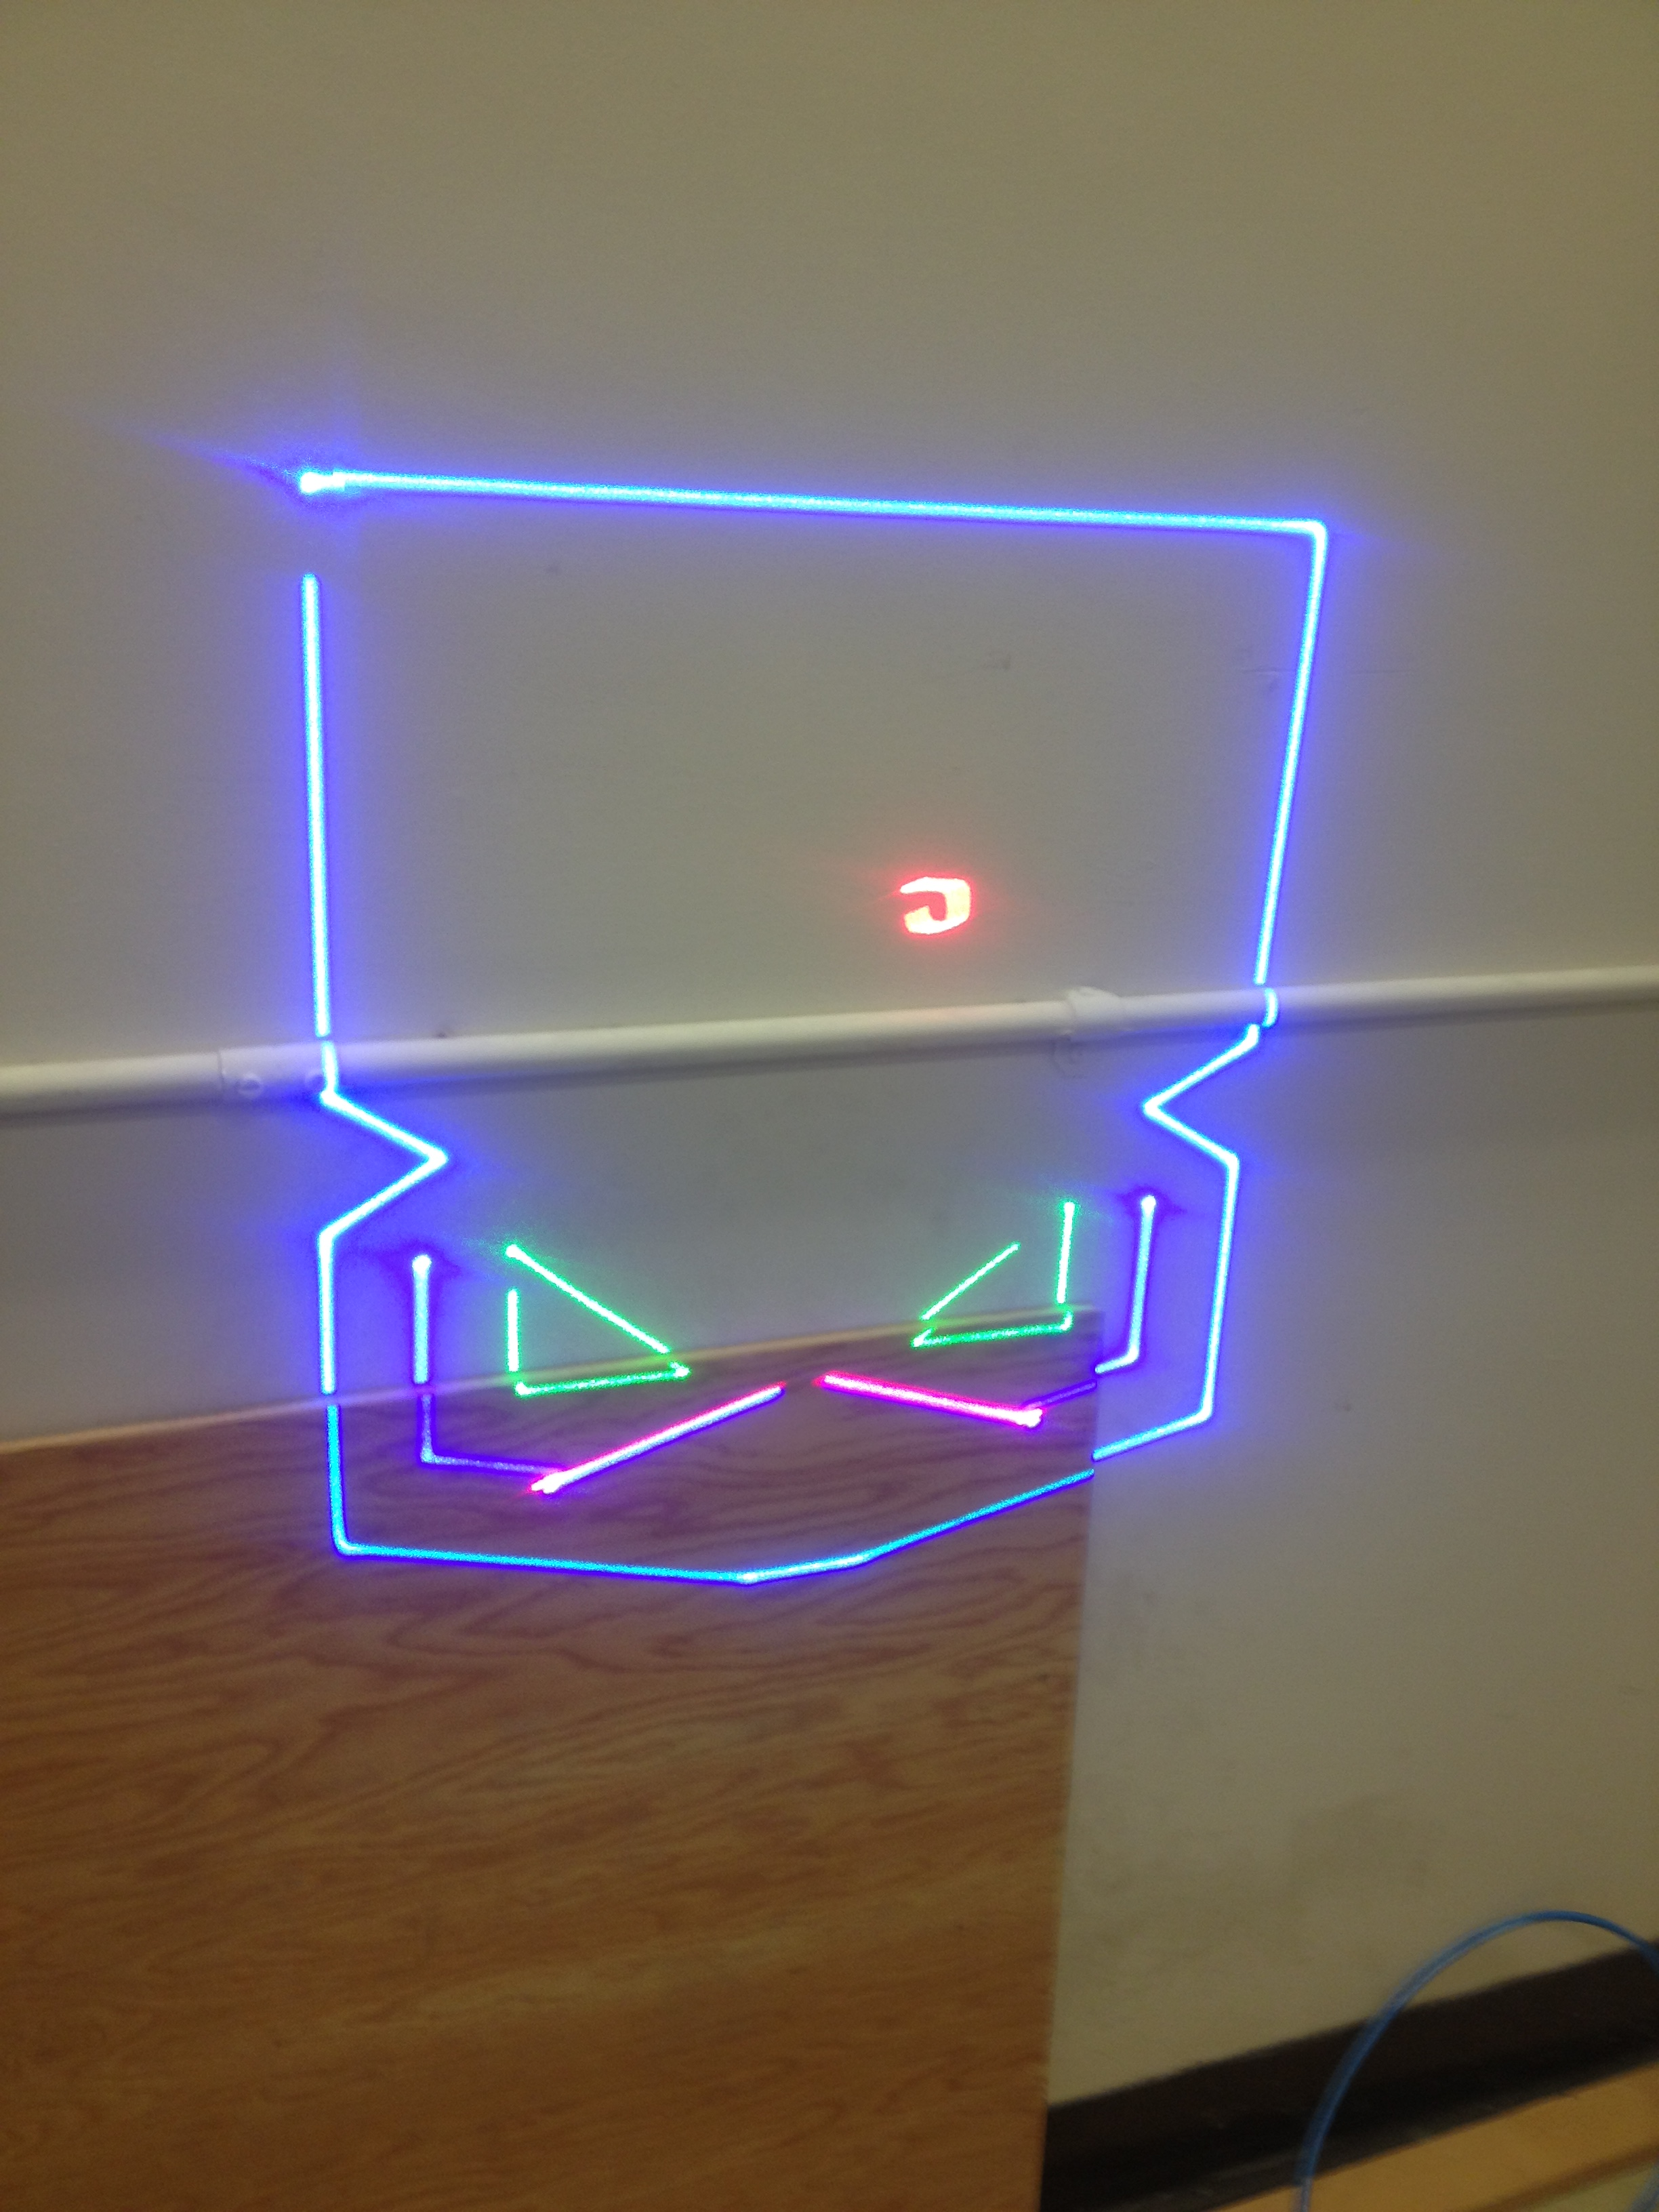
\includegraphics[width=.6\linewidth]{laser_success}
  \caption{Adding corner stalls to sharpen corners and wait periods for laser power toggle.}
\end{minipage}
\end{figure}

We also encountered less common issues, such as one of our first figures being rotated by 90$\degree$ because of a swapped pair of wires on the board. Additionally, an error in the schematic for the laser control board resulted in a limited rotation field for the galvos--the board couldn't drive negative voltage and so was clipping the reachable field to the lower right quadrant. This resulted in our first few tests being much smaller than expected given the values we were sending to the galvos. Coding bugs (like underflow and overflow) also became painfully obvious during laser display testing.

\begin{figure}[H]
\centering
\begin{minipage}{.5\textwidth}
  \captionsetup{width=0.8\textwidth}
  \centering
  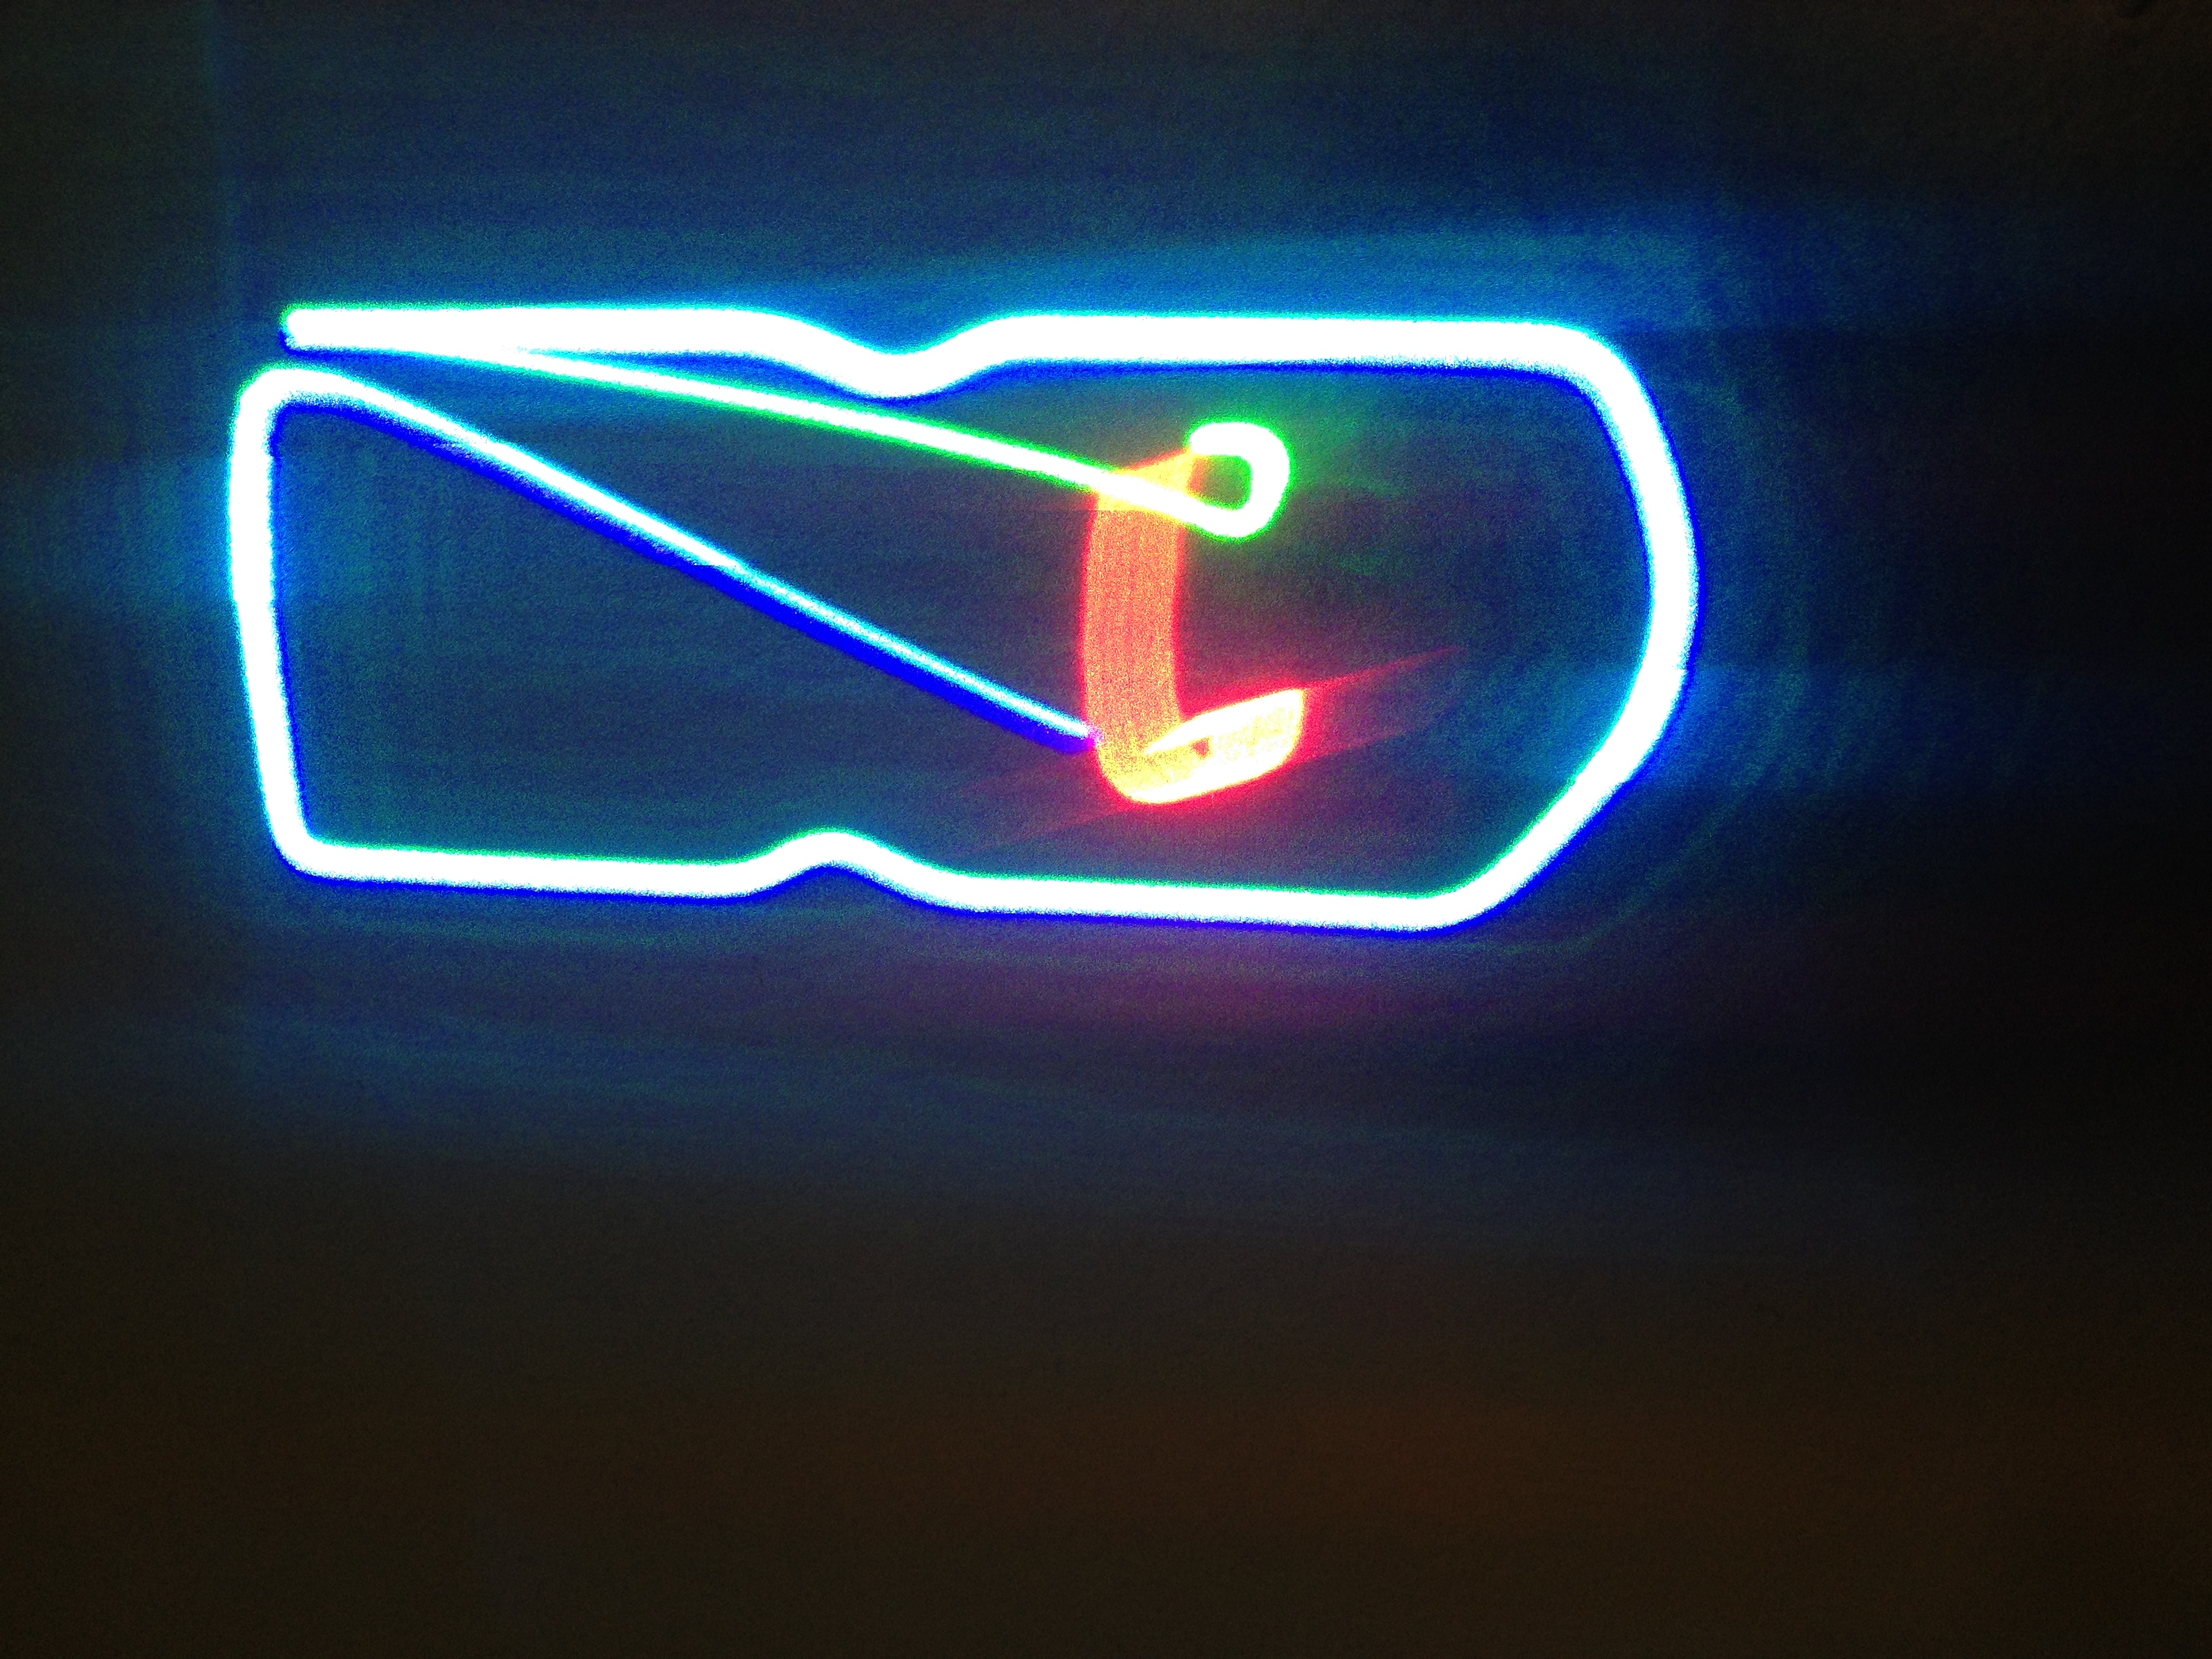
\includegraphics[height=2in]{laser_rotated}
  \caption{One of the first laser tests, both small and rotated.}
\end{minipage}%
\begin{minipage}{.5\textwidth}
  \captionsetup{width=0.8\textwidth}
  \centering
  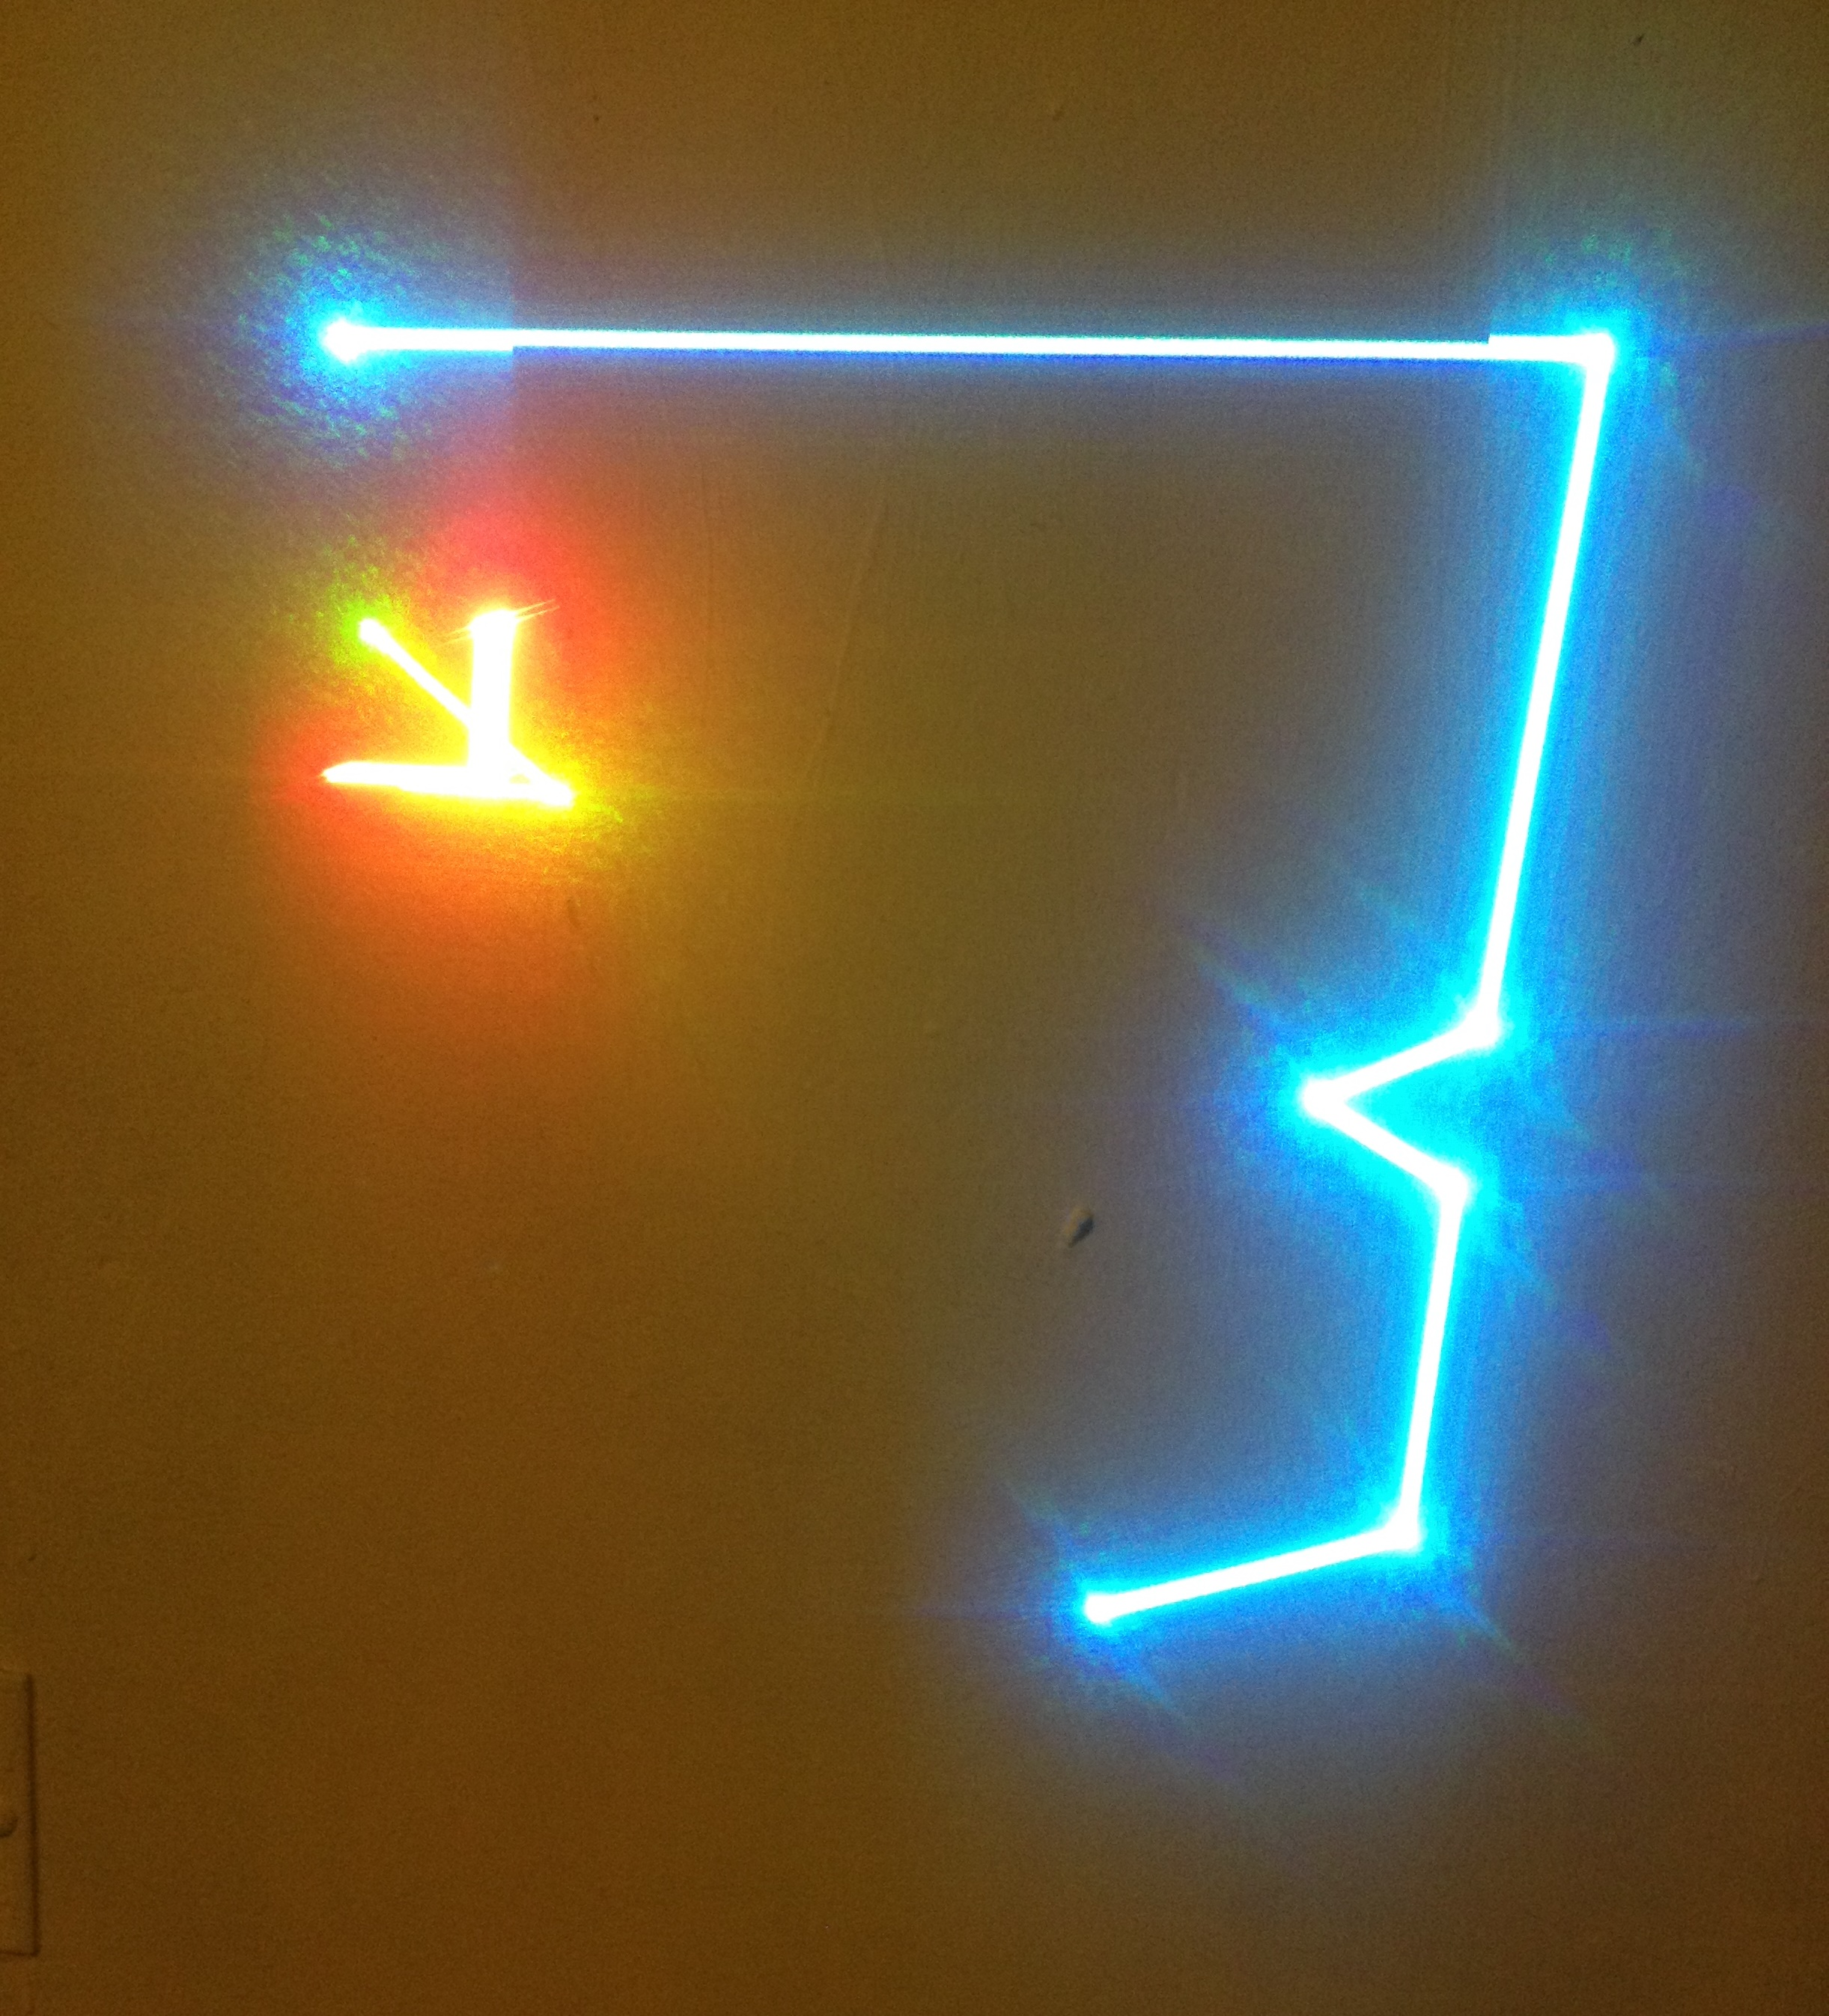
\includegraphics[height=2in]{laser_derp}
  \caption{An assembly bug resulting in the drawing of only half of a sprite.}
\end{minipage}
\end{figure}

\begin{figure}[H]
\centering
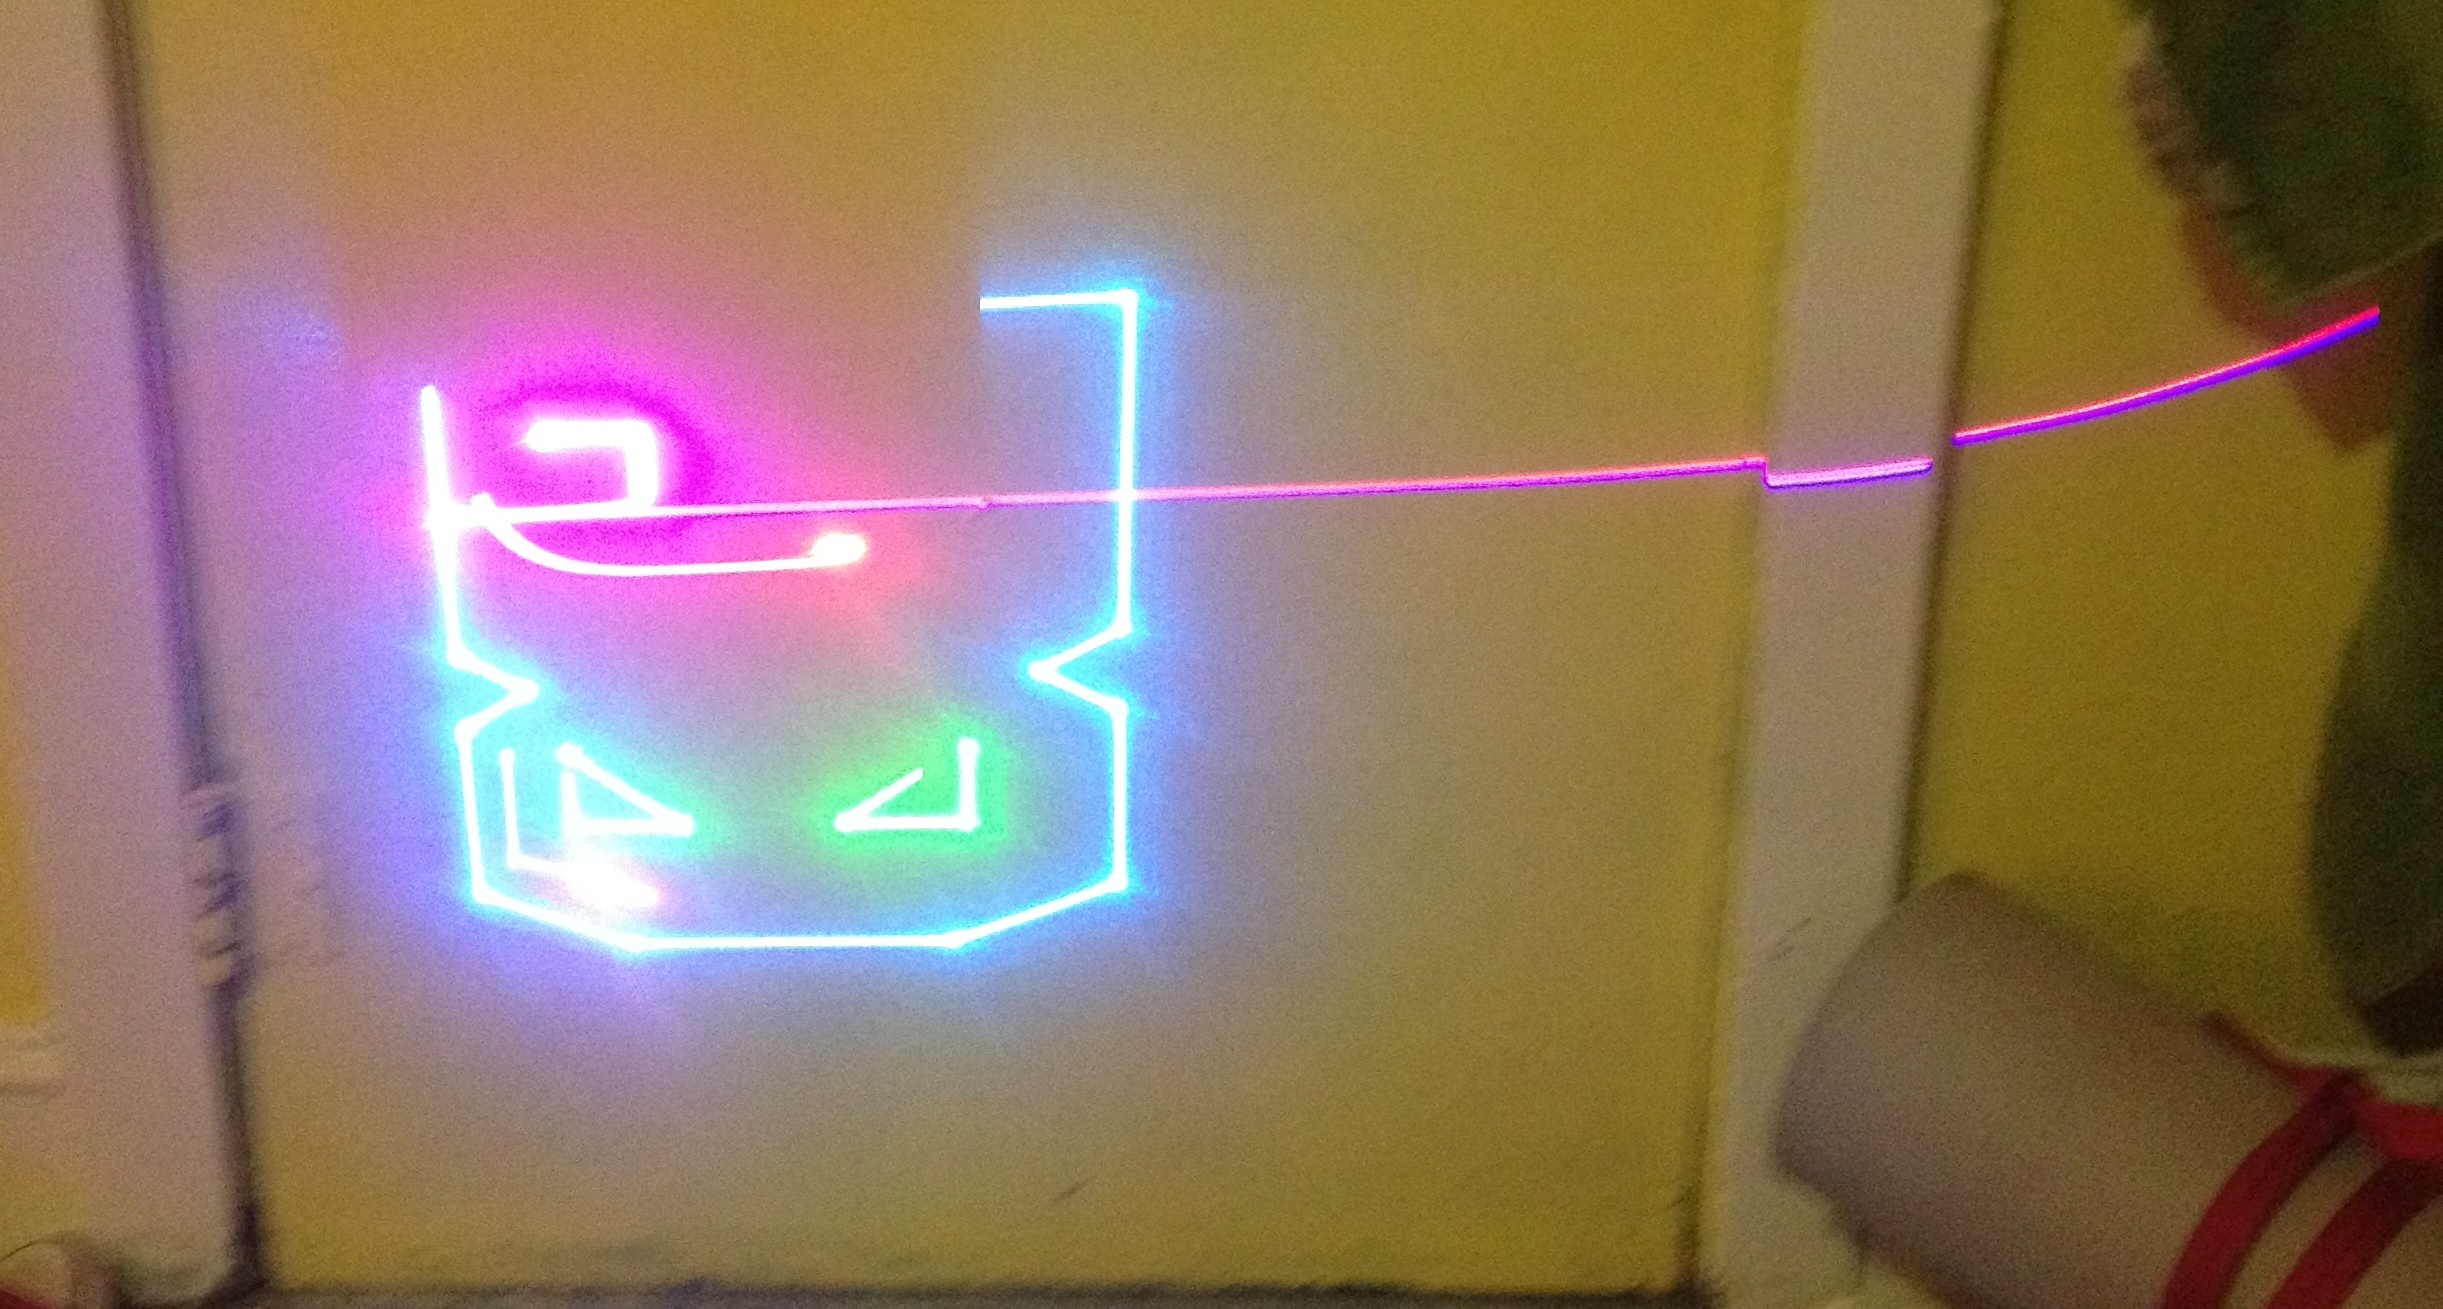
\includegraphics[width=0.5\textwidth]{laser_underflow}
\caption{Problematic register underflow causing the laser beam to shoot to the maximum extent of its range.}
\end{figure}

\subsubsection{Testing}

Testing the laser driver would have been impossible without the 6.004 testing program BSIM. With BSIM we were able to step through the assembly program and verify that it was doing exactly what we wanted it to. This was most helpful in the drawing of the sprites; mapping each sprite to a list of signed hexadecimal offsets by hand was highly prone to error, which caused problematic overflow and underflow as in the figures above. 

\section{Implementation Process} \label{implementation}
\subsection{The $\mu$Beta Processor} \label{mbeta}
The $\mu$Beta processor was based on the two-stage Beta from the old 6.111 course website.  First, the core was modified to have correct register initialization values to allow for simulation in ModelSim. We then discovered that the BEQ and BNE opcodes were incorrect, and fixed them. We added multiply to the Beta and remapped the memory space. 

We also replaced the original memory mapping of the beta and added a shared memory space as well as memory-mapped I/O to turn it into a real microcontroller. Our memory-mapped I/O consisted of two 32 bit wide input ports, two 32 bit wide output ports, SPI, and a timer capable of triggering Beta interrupts. The operating frequency and number of bits to be transmitted for the SPI were both fully configurable though register settings. The timer period and interrupt enable could both be set from register settings and an overflow flag can be both read and cleared. 

Timing analysis of the $\mu$Beta processor revealed that it could be operated at slightly below 100MHz on the Virtex-5 FPGA used in the project with a few extra edits, but we chose to clock it at 50MHz to avoid any undesirable effects resulting from a faster clock speed. 

We found that we could build a large number of 2-stage pipeline \gls{Beta} cores on our Virtex-5 board (almost 40). However, the number of processors that can feasibly be used is limited more realistically by the amount of memory each processor needs for program memory and storage. The two Beta cores that we used were given 16k words of memory each (implemented using BRAM), which proved to be sufficient with ample grow room for future modifications. The 50MHz clock speed chosen was more than adequate for our needs. Due to the physical limitations of our galvanometers, the highest estimate we could make for our frame rate was around 20Hz. In the Beta, all instructions are executed in a single cycle; running at 50MHz, we wouldn't have to worry about meeting our frame rate requirements.

To program the Betas, we needed to pre-load the program memory with .coe files detailing the assembled instructions. Conveniently, the 6.004 BSIM program, readily available on the 6.004 course website, outputs both .bin and .coe files. The latter format is a list of comma-delimited hex values which represent the compiled Beta assembly code, which can be used to compile memories for use in Verilog modules by the ISE CoreGen program. With these memory files converted into memories for the Verilog Beta to read, we were able to simulate the Beta running through arbitrary code in ModelSim. Together with the infinitely useful BSIM simulation module that comes free with your copy of the 6.004 Beta assembler, our Verilog test benches proved invaluable to our testing process.

\subsection{Debugging the OV7670 Camera} \label{camerasuck}

The use of the OV7670 camera in this project became a major hindrance. The cameras are poorly documented, poorly constructed, and require extensive setup; the default configuration settings were unusable, as we needed the camera to output data in RGB format. This required writing configuration registers over I2C. When put into RGB mode image first displayed green as red, red as green, and blue as black. Many hours were spent debugging the camera frame capture Verilog before it was discovered (after much searching the Internet for answers) that the inverted colors were a configuration issue and not an issue with any of the project's Verilog. The C source code for a Linux driver was found for the camera and many of the configuration values were copied from this file. As a testament to the uselessness of the original camera, many of the registers written to were marked as reserved in the data sheet with no other documentation given. Even using the configuration settings found outline, the camera image was of poor quality, which made image recognition difficult.

\subsection{Building a Laser Projector} \label{laserbox}

The laser projector was built inside a project box scavenged from the Stata loading dock with new front, top, and bottom panels designed in SolidWorks and lasercut. We ordered the cheapest RGB laser and galvos we could off of eBay, which proved sufficient for the project. The main issue with these was the lack of mounting holes in the power supplies and galvo drivers. Luckily, liberal application of double-sided sticky tape solved the problem. 

\subsection{Xilinx ML505 FPGA Board} \label{board}

In lieu of the 6.111 labkit, our project used a ML505 Virtex 5 FPGA board that a team member acquired from a previous internship. The Virtex 5 FPGA on this board has only a slightly smaller gate count than the the Virtex-II used on the labkit. This is in comparison to the other common FPGA boards, which typically have much smaller gate counts.

Using our own FPGA board allowed us to work on the project at any time and place of our choosing and to build the FPGA into the laser projector. However, using this board came with its own set of challenges. Unlike the student-targeted boards that Digilent and other companies make, the ML505 had no examples on how to use any of the interfaces other than pin assignments and part numbers. As a consequence, getting interfaces like VGA up and running took several days. Once over the biggest hump of the learning curve, however, we were able to use the board quite competently to implement what we needed. 

\section{Review and Recommendation}

As is likely obvious, we deeply underestimated the complexity of this project. Things that we assumed would be quick---like getting the camera working at a basic level, for example---ended up taking us weeks of work. We realized fairly late in the game that our project really required a processor; though we did manage to get a working Beta implementation, it took up so much of our time that we had little time left to work on the relevant parts of our project (object recognition, physics, and laser control). It's no surprise, then, that we didn't finish all parts of our project. Thinking back, we should have been less ambitious and scrapped the camera section entirely. Without having to fight with the camera and deal with vision processing, we would have had enough time to generate a working physics engine and laser controller, even with the necessary Beta implementation.

On the plus side, though, implementing the Beta processor on an FPGA did teach us a lot. It was also truly amazing to be able to write code in assembly, load it into BRAM, and watch the processor behave as expected. Even things like simulating in ModelSim were exciting since we were effectively simulating a multicore processor at the gate level. 

\begin{figure}[h]
\centering
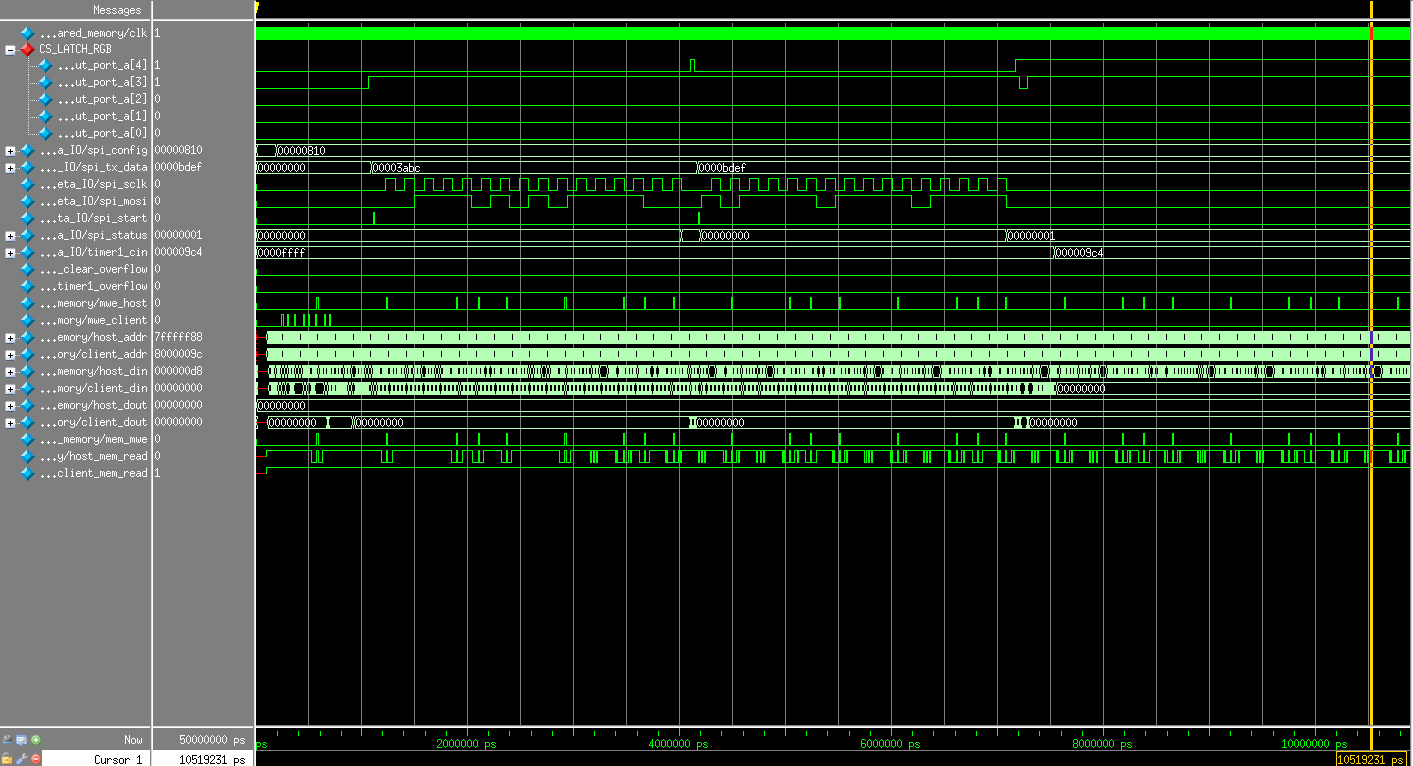
\includegraphics[width=\textwidth]{physics_laser_interact_test01}
\caption{The first test with the two Betas interacting correctly. You can see the SPI transmission occurring and the two Betas (the physics Beta as the host and the laser Beta as the client) using the shared memory space.}
\end{figure}

And once we implemented the Beta processor we actually did manage to get fairly close to completing all parts of our project. With an extra week, we likely could have finished, even with the hangups from the camera---had we initially decided on a multicore Beta architecture rather than restarting halfway through the project we would have made much more progress towards our original goal.

One thing that would have helped tremendously (and could help in the future, if further iterations of this project are attempted) was a C-to-Beta-assembly compiler. Because the Beta instruction set is non-standard, no such industry-standard compiler exists and past students have relied on a compiler that is no longer maintained by its authors. Our attempts to revive this compiler for use on modern systems failed, but if we had had a compiler writing the physics engine would have been comparatively trivial. Fixed-point math in assembly language is not in any way intuitive and would have been much easier in a high-level language like C.

Something else that could have sped up out testing process was a custom bootloader for the Betas on the FPGA. In order to test new code, we had to rebuild the two 16k word program memories (BRAMs) in ISE, then rebuild the entire project. This process took about 15 to 20 minutes, which held up our code testing frequently. Though we thoroughly simulated in both BSIM and ModelSim, one of our biggest sources of error was the physical system itself, which could only be tested by running the assembly code. Had we been able to serially load in a memory initialization, we would have been able to test code on the system much more often without having to rebuild the entire project.


\section{Conclusion}
All things considered, our project came together surprisingly well. Though not all elements of the project were integrated, most of them were fully functional as of the checkoff. The only exception to this was the physics engine, which was close to functional but not yet fully debugged. Though our pinball game is unplayable, the fact that we managed to design object recognition software with a terrible camera and build effectively a commercial laser projector (to display a gameboard with controllable paddles) is fairly amazing. While we're disappointed that we weren't able to get everything finished, we are extremely proud of the work that we did pull together.

And, of course, we achieved our goal of making something really cool---a 400mW laser projecting a pinball board and an SNES controller to toggle the paddles is nothing to scoff at.

\pagebreak
\section{Code}
\subsection{Beta Instruction Set}
\begin{lstlisting}
||||||||||||||||||||||||||||||||||||||||||||||||||||||||||||||||||||||||
||| 6.004 BETA Macro package -                  revised 9/28/11 SAW  |||
|||  This file defines our 32-bit Beta instruction set.              |||
||||||||||||||||||||||||||||||||||||||||||||||||||||||||||||||||||||||||

| Global instruction definition conventions:
|  * DESTINATION arg is LAST

| Instruction set summary.  Notation:
| ra, rb, rc: registers
|         CC: 16-bit signed constant
|      label: statement/location tag (becomes PC-relative offset)

| ADD(RA, RB, RC)	| RC <- <RA> + <RB>
| ADDC(RA, C, RC)	| RC <- <RA> + C
| AND(RA, RB, RC)	| RC <- <RA> & <RB>
| ANDC(RA, C, RC)	| RC <- <RA> & C
| MUL(RA, RB, RC)	| RC <- <RA> * <RB>
| MULC(RA, C, RC)	| RC <- <RA> * C
| DIV(RA, RB, RC)	| RC <- <RA> / <RB>
| DIVC(RA, C, RC)	| RC <- <RA> / C
| OR( RA, RB, RC)	| RC <- <RA> | <RB>
| ORC(RA,  C, RC)	| RC <- <RA> | C
| SHL(RA, RB, RC)	| RC <- <RA> << <RB>
| SHLC(RA, C, RC)	| RC <- <RA> << C
| SHR(RA, RB, RC)	| RC <- <RA> >> <RB>
| SHRC(RA, C, RC)	| RC <- <RA> >> C
| SRA(RA, RB, RC)	| RC <- <RA> >> <RB>
| SRAC(RA, C, RC)	| RC <- <RA> >> C
| SUB(RA, RB, RC)	| RC <- <RA> - <RB>
| SUBC(RA, C, RC)	| RC <- <RA> - C
| XOR(RA, RB, RC)	| RC <- <RA> ^ <RB>
| XORC(RA, C, RC)	| RC <- <RA> ^ C
| XNOR(RA, RB, RC)	| RC <- ~(<RA> ^ <RB>)
| XNORC(RA, C, RC)	| RC <- ~(<RA> ^ C)

| CMPEQ(RA, RB, RC)	| RC <- <RA> == <RB>
| CMPEQC(RA, C, RC)	| RC <- <RA> == C
| CMPLE(RA, RB, RC)	| RC <- <RA> <= <RB>
| CMPLEC(RA, C, RC)	| RC <- <RA> <= C
| CMPLT(RA, RB, RC)	| RC <- <RA> <  <RB>
| CMPLTC(RA, C, RC)	| RC <- <RA> <  C


| BR(LABEL,RC)		| RC <- <PC>+4; PC <- LABEL (PC-relative addressing)
| BR(LABEL)		| PC <- LABEL (PC-relative addressing)
| BEQ(RA, LABEL, RC)	| RC <- <PC>+4; IF <RA>==0 THEN PC <- LABEL
| BEQ(RA, LABEL)	| IF <RA>==0 THEN PC <- LABEL
| BF(RA, LABEL, RC)	| RC <- <PC>+4; IF <RA>==0 THEN PC <- LABEL
| BF(RA, LABEL)		| IF <RA>==0 THEN PC <- LABEL
| BNE(RA, LABEL, RC)	| RC <- <PC>+4; IF <RA>!=0 THEN PC <- LABEL
| BNE(RA, LABEL)	| IF <RA>!=0 THEN PC <- LABEL
| BT(RA, LABEL, RC)	| RC <- <PC>+4; IF <RA>!=0 THEN PC <- LABEL
| BT(RA, LABEL)		| IF <RA>!=0 THEN PC <- LABEL
| JMP(RA, RC)		| RC <- <PC>+4; PC <- <RA> & 0xFFFC
| JMP(RB)		| PC <- <RB> & 0xFFFC

| LD(RA, CC, RC)	| RC <- <<RA>+CC>
| LD(CC, RC)		| RC <- <CC>
| ST(RC, CC, RA)	| <RA>+CC <- <RC>
| ST(RC, CC)		| CC <- <RC>
| LDR(CC, RC)		| RC <- <CC> (PC-relative addressing)

| MOVE(RA, RC)		| RC <- <RA>
| CMOVE(CC, RC)		| RC <- CC
| HALT()		| STOPS SIMULATOR.

| PUSH(RA)		| (2) <SP> <- <RA>; SP <- <SP> - 4
| POP(RA)		| (2) RA <- <<SP>+4>; SP <- <SP> + 4
| ALLOCATE(N)		| Allocate N longwords from stack
| DEALLOCATE(N)		| Release N longwords

| CALL(label)		| Call a subr; save PC in lp.
| CALL(label, n)	| (2) Call subr at label with n args.
			| Saves return adr in LP.
			| Pops n longword args from stack.

| RTN()			| Returns to adr in <LP> (Subr return)
| XRTN()		| Returns to adr in <IP> (Intr return)

| WORD(val)		| Assemble val as a 16-bit datum
| LONG(val)		| Assemble val as a 32-bit datum
| STORAGE(NWORDS)	| Reserve NWORDS 32-bit words of DRAM

| GETFRAME(F, RA)	| RA <- <<BP>+F>
| PUTFRAME(RA, F)	| <BP>+F <- <RA>

| Calling convention:
|	PUSH(argn-1)
|	...
|	PUSH(arg0)
|	CALL(subr, nargs)
|	(return here with result in R0, args cleaned)

| Extra register conventions, for procedure linkage:
| LP = 28			| Linkage register (holds return adr)
| BP = 29			| Frame pointer (points to base of frame)

| Conventional stack frames look like:
|	arg[N-1]
|	...
|	arg[0]
|	<saved lp>
|	<saved bp>
|	<other saved regs>
|   BP-><locals>
|       ...
|   SP->(first unused location)

| Convention: define a symbol for each arg/local giving bp-relative offset.
| Then use
|   getframe(name, r) gets value at offset into register r.
|   putframe(r, name) puts value from r into frame at offset name


||||||||||||||||||||||||||||||||||||||||||||||||||||||||||||||||||||||||
||| End of documentation.  Following are the actual definitions...   |||
||||||||||||||||||||||||||||||||||||||||||||||||||||||||||||||||||||||||

| Assemble words, little-endian:
.macro WORD(x) x%0x100 (x>>8)%0x100 
.macro LONG(x) WORD(x) WORD(x >> 16)	| little-endian for Maybe
.macro STORAGE(NWORDS)	. = .+(4*NWORDS)| Reserve NWORDS words of RAM


| register designators
| this allows symbols like r0, etc to be used as
| operands in instructions. Note that there is no real difference
| in this assembler between register operands and small integers.

r0 = 0
r1 = 1
r2 = 2
r3 = 3
r4 = 4
r5 = 5
r6 = 6
r7 = 7
r8 = 8
r9 = 9
r10 = 10
r11 = 11
r12 = 12
r13 = 13
r14 = 14
r15 = 15
r16 = 16
r17 = 17
r18 = 18
r19 = 19
r20 = 20
r21 = 21
r22 = 22
r23 = 23
r24 = 24
r25 = 25
r26 = 26
r27 = 27
r28 = 28
r29 = 29
r30 = 30
r31 = 31

bp = 27			| frame pointer (points to base of frame)
lp = 28			| linkage register (holds return adr)
sp = 29			| stack pointer (points to 1st free locn)
xp = 30			| interrupt return pointer (lp for interrupts)


| understand upper case, too.
R0 = r0
R1 = r1
R2 = r2
R3 = r3
R4 = r4
R5 = r5
R6 = r6
R7 = r7
R8 = r8
R9 = r9
R10 = r10
R11 = r11
R12 = r12
R13 = r13
R14 = r14
R15 = r15
R16 = r16
R17 = r17
R18 = r18
R19 = r19
R20 = r20
R21 = r21
R22 = r22
R23 = r23
R24 = r24
R25 = r25
R26 = r26
R27 = r27
R28 = r28
R29 = r29
R30 = r30
R31 = r31
XP = xp
LP = lp
BP = bp
SP = sp

.macro betaop(OP,RA,RB,RC) {
      .align 4
      LONG((OP<<26)+((RC%0x20)<<21)+((RA%0x20)<<16)+((RB%0x20)<<11)) }

.macro betaopc(OP,RA,CC,RC) {
      .align 4
      LONG((OP<<26)+((RC%0x20)<<21)+((RA%0x20)<<16)+(CC%0x10000)) }


.macro ADD(RA, RB, RC)		betaop(0x20,RA,RB,RC)
.macro ADDC(RA, C, RC)		betaopc(0x30,RA,C,RC)

.macro AND(RA, RB, RC)		betaop(0x28,RA,RB,RC)
.macro ANDC(RA, C, RC)		betaopc(0x38,RA,C,RC)
.macro MUL(RA, RB, RC)		betaop(0x22,RA,RB,RC)
.macro MULC(RA, C, RC)		betaopc(0x32,RA,C,RC)
.macro DIV(RA, RB, RC)		betaop(0x23,RA,RB,RC)
.macro DIVC(RA, C, RC)		betaopc(0x33,RA,C,RC)
.macro OR( RA, RB, RC)		betaop(0x29,RA,RB,RC)
.macro ORC(RA,  C, RC)		betaopc(0x39,RA,C,RC)
.macro SHL(RA, RB, RC)		betaop(0x2C,RA,RB,RC)
.macro SHLC(RA, C, RC)		betaopc(0x3C,RA,C,RC)
.macro SHR(RA, RB, RC)		betaop(0x2D,RA,RB,RC)
.macro SHRC(RA, C, RC)		betaopc(0x3D,RA,C,RC)
.macro SRA(RA, RB, RC)		betaop(0x2E,RA,RB,RC)
.macro SRAC(RA, C, RC)		betaopc(0x3E,RA,C,RC)
.macro SUB(RA, RB, RC)		betaop(0x21,RA,RB,RC)
.macro SUBC(RA, C, RC)		betaopc(0x31,RA,C,RC)
.macro XOR(RA, RB, RC)		betaop(0x2A,RA,RB,RC)
.macro XORC(RA, C, RC)		betaopc(0x3A,RA,C,RC)
.macro XNOR(RA, RB, RC)		betaop(0x2B,RA,RB,RC)
.macro XNORC(RA, C, RC)		betaopc(0x3B,RA,C,RC)

.macro CMPEQ(RA, RB, RC)	betaop(0x24,RA,RB,RC)
.macro CMPEQC(RA, C, RC)	betaopc(0x34,RA,C,RC)
.macro CMPLE(RA, RB, RC)	betaop(0x26,RA,RB,RC)
.macro CMPLEC(RA, C, RC)	betaopc(0x36,RA,C,RC)
.macro CMPLT(RA, RB, RC)	betaop(0x25,RA,RB,RC)
.macro CMPLTC(RA, C, RC)	betaopc(0x35,RA,C,RC)

.macro BETABR(OP,RA,RC,LABEL)	betaopc(OP,RA,((LABEL-.)>>2)-1, RC)
.macro BEQ(RA, LABEL, RC)	BETABR(0x1C,RA,RC,LABEL)
.macro BEQ(RA, LABEL)		BETABR(0x1C,RA,r31,LABEL)
.macro BF(RA, LABEL, RC)	BEQ(RA,LABEL,RC)
.macro BF(RA,LABEL)		BEQ(RA,LABEL)
.macro BNE(RA, LABEL, RC)	BETABR(0x1D,RA,RC,LABEL)
.macro BNE(RA, LABEL)		BETABR(0x1D,RA,r31,LABEL)
.macro BT(RA,LABEL,RC)		BNE(RA,LABEL,RC)
.macro BT(RA,LABEL)		BNE(RA,LABEL)
.macro BR(LABEL,RC)		BEQ(r31, LABEL, RC)
.macro BR(LABEL)		BR(LABEL, r31)
.macro JMP(RA, RC)		betaopc(0x1B,RA,0,RC)
.macro JMP(RA)			betaopc(0x1B,RA,0,r31)

.macro LD(RA, CC, RC)		betaopc(0x18,RA,CC,RC)
.macro LD(CC, RC)		betaopc(0x18,R31,CC,RC)
.macro ST(RC, CC, RA)		betaopc(0x19,RA,CC,RC)
.macro ST(RC, CC)		betaopc(0x19,R31,CC,RC)
.macro LDR(CC, RC)		BETABR(0x1F, R31, RC, CC)

.macro MOVE(RA, RC)		ADD(RA, R31, RC)
.macro CMOVE(CC, RC)		ADDC(R31, CC, RC)

.macro PUSH(RA)		ADDC(SP,4,SP)  ST(RA,-4,SP)
.macro POP(RA)		LD(SP,-4,RA)   ADDC(SP,-4,SP)

.macro CALL(label)	BR(label, LP)
			
.macro RTN()		JMP(LP)
.macro XRTN()		JMP(XP)

| Controversial Extras
| Calling convention:
|	PUSH(argn-1)
|	...
|	PUSH(arg0)
|	CALL(subr, nargs)
|	(return here with result in R0, args cleaned)

| Extra register conventions, for procedure linkage:
| LP = 28			| Linkage register (holds return adr)
| BP = 29			| Frame pointer (points to base of frame)

| Conventional stack frames look like:
|	arg[N-1]
|	...
|	arg[0]
|	<saved lp>
|	<saved bp>
|	<other saved regs>
|   BP-><locals>
|       ...
|   SP->(first unused location)

| Convention: define a symbol for each arg/local giving bp-relative offset.
| Then use
|   getframe(name, r) gets value at offset into register r.
|   putframe(r, name) puts value from r into frame at offset name


.macro GETFRAME(OFFSET, REG) LD(bp, OFFSET, REG)
.macro PUTFRAME(REG, OFFSET) ST(REG, OFFSET, bp)
.macro CALL(S,N) BR(S,lp) SUBC(sp, 4*N, sp)

.macro ALLOCATE(N) ADDC(sp, N*4, sp)
.macro DEALLOCATE(N) SUBC(sp, N*4, sp)

|--------------------------------------------------------
| Privileged mode instructions
|--------------------------------------------------------

.macro PRIV_OP(FNCODE)		betaopc (0x00, 0, FNCODE, 0)
.macro HALT() PRIV_OP (0)
.macro RDCHAR() PRIV_OP (1)
.macro WRCHAR() PRIV_OP (2)
.macro CYCLE()	PRIV_OP (3)
.macro TIME()	PRIV_OP (4)
.macro CLICK()	PRIV_OP (5)
.macro RANDOM()	PRIV_OP (6)
.macro SEED()	PRIV_OP (7)
.macro SERVER() PRIV_OP (8)

| SVC calls; used for OS extensions

.macro SVC(code)		betaopc (0x01, 0, code, 0)

| Trap and interrupt vectors
VEC_RESET	= 0		| Reset (powerup)
VEC_II		= 4		| Illegal instruction (also SVC call)
VEC_CLK		= 8		| Clock interrupt
VEC_KBD		= 12		| Keyboard interrupt
VEC_MOUSE	= 16		| Mouse interrupt

| constant for the supervisor bit in the PC
PC_SUPERVISOR	   = 0x80000000		| the bit itself
PC_MASK            = 0x7fffffff		| a mask for the rest of the PC
\end{lstlisting}

\subsection{Laser Controller Assembly}
\begin{lstlisting}
.include beta.uasm

| REGISTER MAP
|	r0:   x location
|	r1:   y location
|	r2:   current sprite id
|	r3:   rgb value for laser
|	r4:   current offset into shared memory
|	r5:   counter
|	r6:   length of sprite
|	r7:   scratch
|	r8:   scratch
|	r9:   current location in local sprite lookup table
|	r10:  spi tx data, daca
|	r11:  spi tx data, dacb
| 	r12:  holds remaining number of points in current segment
|	r13:  scratch
|	r14:  scale factor - currently inactive
|	r15:  laser power flag for implementing travels
|	r16:  reserved for copy of rgb data
|	r17:  scratch
|	r18:  scratch
| 	r19:  holds scaling factor
|	r20:  travel time
|	r21:  stall time


| Define parameters
NEXT_SPRITE_OFFSET = 0x04
|TIMER_VALUE = 0x0D05		| 15kHz
TIMER_VALUE = 0x09C4			| 20kHz
|TIMER_VALUE = 0x01			| DEBUG

| External address offsets
SPI_CONFIG = 0x10
SPI_STATUS = 0x14
INPUT_PORT_A = 0x0
DAC_CTL_OUT = 0x08
SPI_TX = 0x18
TIMER_SET = 0x24
TIMER_OVERFLOW = 0x2C
SHARED_MEM_WRITE_STATUS = 0x100
SHARED_MEM_READ_STATUS = 0x101
SWITCHES = 0x00
STALL_TIME = 0x04					| DEBUG
TRAVEL_TIME = 0x16				| DEBUG
SCALING_FACTOR = 0x0				| full scale (DEBUG)
|SCALING_FACTOR = 0x1			| half scale (DEBUG)
LEFT_PADDLE_UPDATE = 0xF8		| location of left and right paddle offset update values
RIGHT_PADDLE_UPDATE = 0xFC


. = 0				
BR(init)

. = 4
INTERRUPT:
ADD(r31, r31, r31)
XRTN()

| Output port B (0008): {ADC_CSN, ADC_latch_n, R, G, B}
| Input port A (0000): { [31:24] TRAVEL_TIME, [23:16] STALL_TIME, [15:8] UNUSED, [7:0] SCALING_FACTOR }

| Initialize sprite location in shared memory, initialize SPI, get scale factor
init:
	CMOVE(stack, SP)					| Initialize stack
	CMOVE(2, r4)						| initialize sprite location in shared memory
	SHLC(r4, 16, r4)
	
	CMOVE(1, r7)						| initialize output port location in shared memory
	SHLC(r7, 16, r7)
	CMOVE(0x0810, r8)					| configure SPI
	ST(r8, SPI_CONFIG, r7)

  	LD(r7, INPUT_PORT_A, r19)		| load input port A into r19
	CMOVE(0xFF, r8)
	SHLC(r8, 24, r8)
	AND(r8, r19, r20)					| load travel time value into r20
	SHRC(r8, 8, r8)
	AND(r8, r19, r21)					| load stall time into r21
	CMOVE(0xFF, r8)
	AND(r8, r19, r19)					| load scaling factor into r19
	
	

| Draws every sprite in a frame
check_data_available:
	LD(r4, SHARED_MEM_WRITE_STATUS, r7)	| check shared memory write status
	BNE(r7, check_data_available)
	CMOVE(1, r7)
	ST(r7, SHARED_MEM_READ_STATUS, r4)		| set the read flag
draw_frame:
	| Load sprite IDs until you find a null-terminated one
	LD(r4, 0, r7) 						| load new sprite data into r7
	SHRC(r7, 27, r2) 					| get just the sprite ID
	BEQ(r2, frame_done) 				| if sprite ID is null then we're done, otherwise continue loading
	
	SUBC(r20, 1, r8) 					| store 0xFFFFFFFF in r8
	SHRC(r8, 8, r8) 					| 0x00FFFFFF in r8
	AND(r7, r8, r0) 					| mask off the sprite ID and RGB data
	SHRC(r0, 12, r0) 					| store only x data in r0
	SHRC(r8, 12, r8) 					| 0x00000FFF in r8
	AND(r7, r8, r1) 					| store only y data in r1
	SHRC(r7, 24, r16) 				| mask off x and y data
	ANDC(r16, 0x07, r16) 			| rgb data in r16
	CALL(draw_sprite)
	
	ADDC(r4, NEXT_SPRITE_OFFSET, r4)	| get next sprite location in shared memory
	
	BR(draw_frame)
	
frame_done:
	CMOVE(2, r4)
	SHLC(r4, 16, r4) 					| clear frame offset (shared memory)
	CMOVE(0, r7)
	ST(r7, SHARED_MEM_READ_STATUS, r4)	| clear busy flag
	
	BR(check_data_available)


|| Start the timer, wait for it to finish, and clear the flag (have to reload counter to reset)
set_timer:
	
	| Initialize and reset timer
	CMOVE(1, r7) 						| store timer address in r7
	SHLC(r7, 16, r7)
	CMOVE(TIMER_VALUE, r8) 			| load for gavlo update frequency
	ST(r8, TIMER_SET, r7)
	
wait_timer:
	LD(r7, TIMER_OVERFLOW, r8)
| update paddles while we're waiting for the timer
	SHLC(r7, 1, r13)								| address into shared memory
	LD(r13, LEFT_PADDLE_UPDATE, r17)			| update left paddle
	ST(r17, left_paddle_hops, r31)
	LD(r13, RIGHT_PADDLE_UPDATE, r17)		| update right paddle
	ST(r17, right_paddle_hops, r31)
|	BNE(r8, wait_timer)							| DEBUG	
	BEQ(r8, wait_timer) 							| flag should be set when timer is done
	CMOVE(0x0, r8) 								| clear flag
	ST(r8, TIMER_OVERFLOW, r7)
	RTN()
|| Draw a single sprite
draw_sprite:
	| Get length of sprite from lookup table, store in r6
	|.breakpoint
	SHLC(r2, 8, r8) 							| translate sprite ID into lookup table offset
	ADDC(r8, sprite_lookup, r9)
	LD(r9, 0, r6) 								| first entry in lookup table is sprite length
	ADDC(r9, 0x4, r9)							| store location of first point for get_next_point routine
  	LD(r9,0x4,r12)    						| load number of points in next segment into r12
  	SHLC(r12, SCALING_FACTOR, r12) 	   | multiply the number of points by the scaling factor 
	CMOVE(0x1, r15)    						| set flag signaling laser turn on after next segment
	
| Draw the sprite:
draw_loop:
	PUSH(LP)
	CALL(go_to_point)
	CALL(get_next_point)
	CALL(set_timer)
	POP(LP)
	
	BNE(r6, draw_loop)
	RTN()
	
|| Go to a single point by writing its location over SPI
go_to_point:
		
	CMOVE(0x02, r8) 						| put SPI address in r8
	SHLC(r8, 16, r8)
  	SHRC(r0,SCALING_FACTOR,r17)		| restore scaling
  	SHRC(r1,SCALING_FACTOR,r18)
	
	ORC(r3, 0b01000, r7) 			| Store CS & RGB data in r7
	CMOVE(0b0011, r10) 				| Store config data (1) in r10
	SHLC(r10, 12, r10) 				| Shift left to bit 15
	OR(r10, r17, r10) 				| r10 now contains config data for write to DACA
	
	CMOVE(0b01011, r11) 				| Store config data (2) in r11
	SHLC(r11, 12, r11) 				| Shift left to bit 15
	OR(r11, r18, r11) 				| r11 now contains config data for write to DACB
	|.breakpoint
	CMOVE(0x01, r8) 					| put SPI address in r8
	SHLC(r8, 16, r8)
	ST(r7, DAC_CTL_OUT, r8) 		| Write to output port A (memory location 8)--lower CS
	ST(r10, SPI_TX, r8) 				| Write configuration and X data to SPI TX (0018)
	
	CMOVE(1, r13) 						| Store 1 (start flag) in r13
	ST(r13, SPI_STATUS, r8) 		| Start SPI
spi_wait_x: 							| Wait for SPI completion flag
	LD(r8, SPI_STATUS, r13)
	BF(r13, spi_wait_x)
	
	ORC(r7, 0b10000, r7)
	ST(r7, DAC_CTL_OUT, r8) 		| Write to output port A (memory location 8)--raise CS
	ADD(r31, r31, r31)
	ANDC(r7, 0b01111, r7)
	
	ST(r7, DAC_CTL_OUT, r8) 		| Write to output port A--lower CS
	ADD(r31, r31, r31)
	ST(r11, SPI_TX, r8) 				| Write configuration and Y data to SPI TX (0018)
	ST(r13, SPI_STATUS, r8) 		| Start SPI
	
spi_wait_y: 							| Wait for second SPI completion flag
	LD(r8, SPI_STATUS, r13)
	BF(r13, spi_wait_y)
	
	ORC(r7, 0b10000, r7)
	ST(r7, DAC_CTL_OUT, r8) 		| Write to output port A (memory location 8)--raise CS
	ADD(r31, r31, r31)
	SUBC(r7, 0b01000, r7)
	ST(r7, DAC_CTL_OUT, r8) 		| Lower ADC latch
	ADD(r31, r31, r31)
	ADD(r31, r31, r31)
	ADD(r31, r31, r31)
	ADD(r31, r31, r31)
	ADDC(r7, 0b01000, r7)
	ST(r7, DAC_CTL_OUT, r8) 		| Raise ADC latch	
	ADD(r31, r31, r31)
	ADD(r31, r31, r31)
	ADD(r31, r31, r31)
	ADD(r31, r31, r31)
	RTN()
	
|| Get the location of the next point within a shape and store the updated location in registers 0 and 1 (x and y)	
get_next_point:

	LD(r9, 0, r8)	 					| load next point into r8
	MOVE(r8, r7)		        		| copy point
  	SUBC(r12,0x1,r12)             | decrement remaining points in the line
	SRAC(r8, 16, r8) 					| Get only x data
	SHLC(r7, 16, r7) 					| Get only y data, preserving sign bit
	SRAC(r7, 16, r7)
	ADD(r8, r0, r0) 					| Add x offset
	ADD(r7, r1, r1) 					| Add y offset
  	BNE(r12, get_next_end)   		| if we're done with this line segment,
    	.breakpoint
    		ADDC(r9, 0x8, r9)       | increment location in local table
    		LD(r9,0x4,r12)          | load point count for next segment
	  	SUBC(r6, 0x01, r6)     		| decrement points left for sprite
    		CMPEQC(r6, 1, r8)       | test to see if we're about to do our last stall
    		
		BEQ(r8, check_laser_flag)   	| if we are, turn the laser off
    		|.breakpoint
      			CMOVE(0x0,r3)     	| turn laser off
      			CMOVE(0x0,r15)    	| clear flag so the laser doesn't turn on during the next stall

check_laser_flag:
  	BEQ(r15, get_next_end)
  	|.breakpoint
    	MOVE(r16,r3)      				| reload RGB data to turn laser back on

get_next_end:
	RTN()


| Sprite lookup tables: one table for each sprite, memory location corresponds to sprite ID
sprite_lookup:
. = sprite_lookup+0x100
LONG(7) 												| a four-pointed circle for the ball: 1
LONG(0x00000000), LONG(TRAVEL_TIME)    	| stall for travel time
LONG(0x00000000), LONG(STALL_TIME)    		| stall for laser on
LONG(0x00100000), LONG(0x08)
LONG(0x00000010), LONG(0x08)
LONG(0xFFF00000), LONG(0x08)
LONG(0x0000FFF0), LONG(0x08)
LONG(0x00000000), LONG(STALL_TIME)

. = sprite_lookup+0x200
LONG(7)												| arbitrary circle (three times bigger): 2
LONG(0x00000000), LONG(TRAVEL_TIME)    	| stall for travel time
LONG(0x00000000), LONG(STALL_TIME)    		| stall for laser on
LONG(0x00300000), LONG(0x08)
LONG(0x00000030), LONG(0x08)
LONG(0xFFD00000), LONG(0x08)
LONG(0x0000FFD0), LONG(0x08)
LONG(0x00000000), LONG(STALL_TIME)

. = sprite_lookup+0x300 						| the frame outline: 3
LONG(26)
LONG(0x00000000), LONG(TRAVEL_TIME)    	| stall for travel time
LONG(0x00000000), LONG(STALL_TIME)    		| stall for laser on
LONG(0x00500000), LONG(0x20)
LONG(0x00000000), LONG(STALL_TIME)
LONG(0x00000030), LONG(0x20)
LONG(0x00000000), LONG(STALL_TIME)
LONG(0xFFD80018), LONG(0x8)
LONG(0x00000000), LONG(STALL_TIME)
LONG(0x00280018), LONG(0x8)
LONG(0x00000000), LONG(STALL_TIME)
LONG(0x00000030), LONG(0x12)
LONG(0x00000000), LONG(STALL_TIME)
LONG(0xFFBA0012), LONG(0x10)
LONG(0x00000000), LONG(STALL_TIME)
LONG(0xFFEC0000), LONG(0x10)
LONG(0x00000000), LONG(STALL_TIME)
LONG(0xFFBAFFEE), LONG(0x10)
LONG(0x00000000), LONG(STALL_TIME)
LONG(0x0000FFD0), LONG(0x12)
LONG(0x00000000), LONG(STALL_TIME)
LONG(0x0028FFE8), LONG(0x8)
LONG(0x00000000), LONG(STALL_TIME)
LONG(0xFFD8FFE8), LONG(0x8)
LONG(0x00000000), LONG(STALL_TIME)
LONG(0x0000FFD0), LONG(0x20)
LONG(0x00000000), LONG(STALL_TIME)    		| stall for laser off

. = sprite_lookup+0x400							| left triangle bumper: 4
LONG(8)
LONG(0x00000000), LONG(TRAVEL_TIME)    	| stall for travel time
LONG(0x00000000), LONG(STALL_TIME)    		| stall for laser on
LONG(0x001E0018), LONG(0x10)
LONG(0x00000000), LONG(STALL_TIME)
LONG(0xFFE20000), LONG(0x10)
LONG(0x00000000), LONG(STALL_TIME)
LONG(0x0000FFE8), LONG(0x10)
LONG(0x00000000), LONG(STALL_TIME)    		| stall for laser off

. = sprite_lookup+0x500							| right triangle bumper: 5
LONG(8)
LONG(0x00000000), LONG(TRAVEL_TIME)    	| stall for travel time
LONG(0x00000000), LONG(STALL_TIME)    		| stall for laser on
LONG(0x00000018), LONG(0x10)
LONG(0x00000000), LONG(STALL_TIME)
LONG(0xFFE20000), LONG(0x10)
LONG(0x00000000), LONG(STALL_TIME)
LONG(0x001EFFE8), LONG(0x10)
LONG(0x00000000), LONG(STALL_TIME)    		| stall for laser off

. = sprite_lookup+0x600			| left bumpery thing: 6
LONG(6)
LONG(0x00000000), LONG(TRAVEL_TIME)
LONG(0x00000000), LONG(STALL_TIME)
LONG(0x00000022), LONG(0x10)
LONG(0x00000000), LONG(STALL_TIME)
LONG(0x00220008), LONG(0x10)
LONG(0x00000000), LONG(STALL_TIME)

. = sprite_lookup+0x700
LONG(6)					| right bumpery thing: 7
LONG(0x00000000), LONG(TRAVEL_TIME)
LONG(0x00000000), LONG(STALL_TIME)
LONG(0x00000022), LONG(0x10)
LONG(0x00000000), LONG(STALL_TIME)
LONG(0xFFDE0008), LONG(0x10)
LONG(0x00000000), LONG(STALL_TIME)

. = sprite_lookup+0x800
LONG(4)					| left paddle: 8
LONG(0x00000000), LONG(TRAVEL_TIME)
LONG(0x00000000), LONG(STALL_TIME)
left_paddle_hops:
LONG(0x00180008), LONG(0x20)
LONG(0x00000000), LONG(STALL_TIME)

. = sprite_lookup+0x900
LONG(4)					| right paddle: 9
LONG(0x00000000), LONG(TRAVEL_TIME)
LONG(0x00000000), LONG(STALL_TIME)
right_paddle_hops:
LONG(0xFFE80008), LONG(0x20)
LONG(0x00000000), LONG(STALL_TIME)


stack:
STORAGE(128)

|.=0x10000				| DEBUG
|LONG(0x1)
|.=0x20000
|LONG(0x1B000000)
|LONG(0x151E01E0)
|LONG(0x0C600400)
|LONG(0x221E07E0)
|LONG(0x2A8207E0)
|.=0x40000
|LONG(0x1EEB)
\end{lstlisting}

\subsection{Physics Engine Assembly}
\subsubsection{Tested Copy for Checkoff: No implemented physics, paddle control only}
\begin{lstlisting}
.include beta.uasm		| Define Beta instructions, etc.
.options clock tty

|========================================================
| REGISTER MAP
| r0: scratch
| r1: sprite ID (five bits)
| r2: position OR angle
| r3: x velocity
| r4: y velocity
| r5: color (RGB)
| r8: instance pointer
| r9: PC
| r10: 
| r15: external base address
| r16: offset external
| r17: argument to write_external
| r18: byte offset sprite ID
|========================================================

POSITION_OFFSET = 0x04
COLOR_OFFSET = 0x10
NEXT_SPRITE_OFFSET = 0x14
L_PADDLE_UPDATE = 0xF8
R_PADDLE_UPDATE = 0xFC

. = 0
BR(start)

. = 0x4
INT_V:
ADDC(R31, 0, R31)
XRTN()

. = 0x10
start:
CMOVE(stack, SP)

CMOVE(0xFFFF,R10)
SHLC(R10, 16, R10)
SHRC(R10, 16, R10)

CMOVE(0x3,R1)
CMOVE(0,R2)
CMOVE(0x7,R3)
CMOVE(0x9,R4)
CMOVE(0x3,R5)
CALL(build_object)	| bounding box: cyan

|CMOVE(0x2,R1)
|CMOVE(0x01E0,R2)
|SHLC(R2,12,R2)
|CMOVE(0x01E0,R0)
|AND(R0,R10,R0)
|ADD(R0,R2,R2)
|CMOVE(0x9,R3)
|CMOVE(0x1,R4)
|CMOVE(0x5,R5)
|CALL(build_object)	| arbitrary circle: purple

CMOVE(0x1,R1)
CMOVE(0x0600,R2)
SHLC(R2,12,R2)
CMOVE(0x0400,R0)
AND(R0,R10,R0)
ADD(R0,R2,R2)
CMOVE(0x9,R3)
CMOVE(0x1,R4)
CMOVE(0x4,R5)
CALL(build_object)	| arbitrary circle (puck): red

CMOVE(0x4,R1)
CMOVE(0x01E0,R2)
SHLC(R2,12,R2)
CMOVE(0x07E0,R0)
AND(R0,R10,R0)
ADD(R0,R2,R2)
CMOVE(0x9,R3)
CMOVE(0x1,R4)
CMOVE(0x2,R5)
CALL(build_object)	| left bumper: green

CMOVE(0x6,R1)
CMOVE(0x00F0,R2)
SHLC(R2,12,R2)
CMOVE(0x07E0,R0)
AND(R0,R10,R0)
ADD(R0,R2,R2)
CMOVE(0x9,R3)
CMOVE(0x1,R4)
CMOVE(0x1,R5)
CALL(build_object)	| left slide thing: blue

CMOVE(0x8,R1)
CMOVE(0x023E,R2)
SHLC(R2,12,R2)
CMOVE(0x0A80,R0)
AND(R0,R10,R0)
ADD(R0,R2,R2)
CMOVE(0x9,R3)
CMOVE(0x1,R4)
CMOVE(0x7,R5)
CALL(build_object)	| left paddle: white

CMOVE(0x5,R1)
CMOVE(0x0820,R2)
SHLC(R2,12,R2)
CMOVE(0x07E0,R0)
AND(R0,R10,R0)
ADD(R0,R2,R2)
CMOVE(0x9,R3)
CMOVE(0x1,R4)
CMOVE(0x2,R5)      	
CALL(build_object)	| right bumper: green

CMOVE(0x7,R1)
CMOVE(0x0910,R2)
SHLC(R2,12,R2)
CMOVE(0x07E0,R0)
AND(R0,R10,R0)
ADD(R0,R2,R2)
CMOVE(0x9,R3)
CMOVE(0x1,R4)
CMOVE(0x1,R5)
CALL(build_object)	| right slide thing: blue

CMOVE(0x9,R1)
CMOVE(0x07C2,R2)
SHLC(R2,12,R2)
CMOVE(0x0A80,R0)
AND(R0,R10,R0)
ADD(R0,R2,R2)
CMOVE(0x9,R3)
CMOVE(0x1,R4)
CMOVE(0x7,R5)
CALL(build_object)	| right paddle: white

loop:
  CALL(update)
  BR(loop)

update:        			| process next game object

update_start:
  LD(instance_list,R8)      | load the current offset into the list
  LD(R8,0,R1)   		        | load SPRITE_ID of next object
  LD(R8,POSITION_OFFSET,R2)	| load POSITION of next object
  LD(R8,COLOR_OFFSET,R5)	  | load RGB of next object

| packet build routine
  SHLC(R1,27,R17)		| shift SPRITE_ID into upper five bits of R17
  SHLC(R5,24,R0)		| shift RGB into bits [26:24] of R17
  ADD(R17,R0,R17)		| combine
  ADD(R17,R2,R17)		| include POSITION: R17 now contains {SPRITE_ID[4:0], RGB[2:0], POSITION_X[11:0], POSITION_Y[11:0]}
|.breakpoint

  PUSH(LP)     			| gotta push LP before you call a function within a function!
  CALL(write_external)
  POP(LP)       		| restore LP
  BNE(R1,cont_update,R31)   	  | if SPRITE_ID != NULL, continue
    CMOVE(instance_list+4,R8)   | reset list pointer
    ST(R8,instance_list)
    CMOVE(0x0,R17)
    CALL(write_external)
    BR(update_start)            | start over
cont_update:
  LD(R8,4,R2) 			          | load coordinates of next object
  SHLC(R1,0x2,R18)           	| turn SPRITE_ID into a byte offset
  LD(R18,object_routines,R18) | LD address of object-specific update routine
  .breakpoint
  JMP(R18, R9)               	| JMP to execute; save PC in R9
  ADDC(R8,NEXT_SPRITE_OFFSET,R8)             	| point list pointer to next next object
  ST(R8,instance_list)
  RTN()

|+========
pinball:
JMP(R9)                     	| return to update function

|+========
r_flipper:
.breakpoint
PUSH(LP)
CALL(paddle_update)
POP(LP)
JMP(R9)                     | return to update function

|+========
l_flipper:
.breakpoint
PUSH(LP)
CALL(paddle_update)
POP(LP)
JMP(R9)                     | return to update function

|+========
tri_bump:
JMP(R9)                     | return to update function

|+========
circ_bump:
JMP(R9)                     | return to update function

|+========
board:
JMP(R9)                     | return to update function

|+========
fixme_1:
JMP(R9)                     | return to update function

|+========
fixme_2:
JMP(R9)                     | return to update function

|+========
fixme_3:
JMP(R9)                     | return to update function

|========================================================
| OBJECT ROUTINE LOOKUP
|   index into list using SPRITE_ID*4
|   load address, then JMP to execute update routine
|=======================================================

object_routines:
  LONG(0xABCD)
  LONG(pinball)
  LONG(r_flipper)
  LONG(l_flipper)
  LONG(tri_bump)
  LONG(circ_bump)
  LONG(board)
  LONG(fixme_1)
  LONG(fixme_2)
  LONG(fixme_3)

|========================================================
| OBJECT INSTANCE LIST STRUCTURE:
|   0x00 pointer to object list: increment by 8 after
|        processing an object
|   0x04 SPRITE_ID - indicates what class of object we are
|        handling
|   0x08 POSITION - x and y data
|   0x0C VEL_X - x velocity
|   0x10 VEL_Y - y velcoity
|   0x14 RGB - sprite color  
|   ...
|   ... list of objects to be processed
|   ...
|   0x4n - NULL
|========================================================

instance_list: LONG(.+4)    | pointer to the object list
  STORAGE(256)              | allocated object memory

|+==========+
| for writing to the memory block shared with the laser projector
|===========
write_external:
  CMOVE(0x3000,R15)
  SHLC(R15,4,R15)     | load R15 with the bottom address of the external mem
  ADD(R15,R16,R15)    | add offset into memory from R16
  ST(R17,0,R15)       | write the contents of R17 into memory
|.breakpoint
  ADDC(R16,4,R16)     | increment offset for next time
  BNE(R17,write_end)
    CMOVE(0x0,R16)    | if we're done with the frame, clear offset
write_end:
  RTN()
|+==========+
| builds an object in the instance_list
| before calling, put the appropriate values in R1-5
|***********
build_object:
  LD(count, R0)
  ADDC(R0,1,R0)                 | increment the count for next time
  ST(R0, count)                 | store the new count back in memory
  SUBC(R0,1,R0)
  MULC(R0,20,R0)                | turn count in R0 into the offset into the object list
  ST(R1,instance_list+4,R0)     | store object attributes
  ST(R2,instance_list+8,R0)
  ST(R3,instance_list+12,R0)
  ST(R4,instance_list+16,R0)
  ST(R5,instance_list+20,R0)
  ST(R31,instance_list+24,R0)   | end list with NULL; gets overwritten by next object
.breakpoint
  RTN()
count: LONG(0x0)      | for storing the object instance count
paddle_update:
	PUSH(r0)
	PUSH(r1)
	PUSH(r2)
	PUSH(r7)
	PUSH(r8)
	CMOVE(0x1, r7) | right paddle mask
	CMOVE(0x2, r8)	| left paddle mask
	
	CMOVE(0x1, r0)
	SHLC(r0, 16, r0)
	LD(r0, 0, r0)		| get value from input port a. lsb is right paddle, second bit is left paddle.
	
	CMOVE(0x3, r1)
	SHLC(r1, 16, r1)
	ORC(r1, 0x00F8, r3)	| left paddle update location
	ORC(r1, 0x00FC, r2) | right paddle update location
	
	AND(r7, r0, r7)
	BEQ(r7, right_paddle_down)
right_paddle_up:
	LD(right_paddle_up_val, r13)
	ST(r13, 0, r2)
	AND(r8, r0, r8)
	BEQ(r8, left_paddle_down)
	BR(left_paddle_up)
right_paddle_down:
	LD(right_paddle_down_val, r13)
	ST(r13, 0, r2)
	AND(r8, r0, r8)
	BEQ(r8, left_paddle_down)
	BR(left_paddle_up)
left_paddle_up:
	LD(left_paddle_up_val, r13)
	ST(r13, 0, r3)
	POP(r8)
	POP(r7)
	POP(r2)
	POP(r1)
	POP(r0)
	RTN()
	
left_paddle_down:
	LD(left_paddle_down_val, r13)
	ST(r13, 0, r3)
	POP(r8)
	POP(r7)
	POP(r2)
	POP(r1)
	POP(r0)
	RTN()
left_paddle_down_val:
LONG(0x00180008)
left_paddle_up_val:
LONG(0x0018FFF8)
right_paddle_down_val:
LONG(0xFFE80008)
right_paddle_up_val:
LONG(0xFFE8FFF8)
stack:
STORAGE(256)
|.=0x10000
|LONG(0xFE000001)
|. = 0x00400000
|LONG(0x1EEB)
\end{lstlisting}

\subsubsection{Untested working copy: Physics control}
\begin{lstlisting}
.include beta.uasm		| Define Beta instructions, etc.
.options clock tty

|========================================================
| REGISTER MAP
| r0: scratch
| r1: sprite ID (five bits)
| r2: position OR angle
| r3: x velocity --- both xvel and yvel are left shifted
| r4: y velocity --- by a byte to give fractional components
| r5: color (RGB)
| r6: accel due to gravity based on timestep
| r8: instance pointer
| r9: PC
| r10: 0x0000FFFF
| r11-14 : scratch
| r15: external base address
| r16: offset external
| r17: argument to write_external
| r18: byte offset sprite ID
|========================================================

t0 = R19
t1 = R20
t2 = R21
t3 = R22
t4 = R23
t5 = R24
t6 = R25
t7 = r26

| Define parameters

TIMER_VALUE = 0x8000   | 1.526 kHz
|TIMER_VALUE = 0x1       | DEBUG

GRAV_FRACT = 0xC        | .75 pixels/second^2 left shifted by a byte
FRACT_SHIFT = 0x8        | otherwise known as 3/4

POSITION_OFFSET = 0x04
COLOR_OFFSET = 0x10
NEXT_SPRITE_OFFSET = 0x14
TIMER_SET = 0x24
TIMER_OVERFLOW = 0x2C
INPUT_PORT_A = 0x0

. = 0
BR(start)

. = 0x4
INT_V:
ADDC(R31, 0, R31)
XRTN()

. = 0x10
start:
CMOVE(stack, SP)

CMOVE(0xFFFF,R10)
SHLC(R10, 16, R10)
SHRC(R10, 16, R10)

CMOVE(0x3,R1)
CMOVE(0,R2)
CMOVE(0x0,R3)
CMOVE(0x0,R4)
CMOVE(0x3,R5)
CALL(build_object)	| bounding box: cyan

CMOVE(0x2,R1)
CMOVE(0x02E0,R2)
SHLC(R2,12,R2)
CMOVE(0x01E0,R0)
AND(R0,R10,R0)
ADD(R0,R2,R2)
CMOVE(0x0,R3)
CMOVE(0x0,R4)
CMOVE(0x5,R5)
CALL(build_object)	| arbitrary circle: purple

CMOVE(0x1,R1)
CMOVE(0x0600,R2)
SHLC(R2,12,R2)
CMOVE(0x0400,R0)
AND(R0,R10,R0)
ADD(R0,R2,R2)
CMOVE(0x0,R3)
CMOVE(0x0,R4)
CMOVE(0x4,R5)
CALL(build_object)	| arbitrary circle (puck): red

CMOVE(0x4,R1)
CMOVE(0x01E0,R2)
SHLC(R2,12,R2)
CMOVE(0x07E0,R0)
AND(R0,R10,R0)
ADD(R0,R2,R2)
CMOVE(0x0,R3)
CMOVE(0x0,R4)
CMOVE(0x2,R5)
CALL(build_object)	| left bumper: green

CMOVE(0x6,R1)
CMOVE(0x00F0,R2)
SHLC(R2,12,R2)
CMOVE(0x07E0,R0)
AND(R0,R10,R0)
ADD(R0,R2,R2)
CMOVE(0x0,R3)
CMOVE(0x0,R4)
CMOVE(0x1,R5)
CALL(build_object)	| left slide thing: blue

CMOVE(0x8,R1)
CMOVE(0x023E,R2)
SHLC(R2,12,R2)
CMOVE(0x0A80,R0)
AND(R0,R10,R0)
ADD(R0,R2,R2)
CMOVE(0x0,R3)
CMOVE(0x0,R4)
CMOVE(0x7,R5)
CALL(build_object)	| left paddle: white

CMOVE(0x5,R1)
CMOVE(0x0820,R2)
SHLC(R2,12,R2)
CMOVE(0x07E0,R0)
AND(R0,R10,R0)
ADD(R0,R2,R2)
CMOVE(0x0,R3)
CMOVE(0x0,R4)
CMOVE(0x2,R5)      	
CALL(build_object)	| right bumper: green

CMOVE(0x7,R1)
CMOVE(0x0910,R2)
SHLC(R2,12,R2)
CMOVE(0x07E0,R0)
AND(R0,R10,R0)
ADD(R0,R2,R2)
CMOVE(0x0,R3)
CMOVE(0x0,R4)
CMOVE(0x1,R5)
CALL(build_object)	| right slide thing: blue

CMOVE(0x9,R1)
CMOVE(0x06F0,R2)
SHLC(R2,12,R2)
CMOVE(0x0A80,R0)
AND(R0,R10,R0)
ADD(R0,R2,R2)
CMOVE(0x0,R3)
CMOVE(0x0,R4)
CMOVE(0x7,R5)
CALL(build_object)	| right paddle: white

loop:
  CALL(set_timer)
  CALL(scan)
  CALL(update)
  BR(loop)

r_bump = R22
l_bump = R24
y_vel = R21
x_vel = R23

scan:
  .breakpoint
  CMOVE(0x1000,R15)
  SHLC(R15,4,R15)     | load R15 with the bottom address of the external mem
  LD(R15,INPUT_PORT_A,R0)

scan_rbump:
  CMOVE(0x0,r_bump)
  ANDC(R0,0x1,R20)
  BEQ(R20, scan_lbump)
    CMOVE(0x1,r_bump)

scan_lbump:
  CMOVE(0x0,l_bump)
  ANDC(R0,0x2,R20)
  BEQ(R20, scan_up)
    CMOVE(0x1,r_bump)

scan_up:
  ANDC(R0,0x4,R20)
  BEQ(R20, scan_rarrow)
    ADDC(y_vel,2,y_vel)

scan_rarrow:
  ANDC(R0,0x8,R20)
  BEQ(R20, scan_down)
    ADDC(x_vel,2,x_vel)

scan_down:
  ANDC(R0,0x10,R20)
  BEQ(R20, scan_larrow)
    SUBC(y_vel,2,y_vel)

scan_larrow:
  ANDC(R0,0x20,R20)
  BEQ(R20, end_scan)
    SUBC(x_vel,1,x_vel)
end_scan:
  RTN()

update:        			| process next game object

update_start:
  LD(instance_list,R8)      | load the current offset into the list
  LD(R8,0,R1)   		        | load SPRITE_ID of next object
  LD(R8,POSITION_OFFSET,R2)	| load POSITION of next object
  LD(R8,COLOR_OFFSET,R5)	  | load RGB of next object

| packet build routine
  SHLC(R1,27,R17)		| shift SPRITE_ID into upper five bits of R17
  SHLC(R5,24,R0)		| shift RGB into bits [26:24] of R17
  ADD(R17,R0,R17)		| combine
  ADD(R17,R2,R17)		| include POSITION: R17 now contains {SPRITE_ID[4:0], RGB[2:0], POSITION_X[11:0], POSITION_Y[11:0]}
|.breakpoint

  PUSH(LP)     			| gotta push LP before you call a function within a function!
  CALL(write_external)
  POP(LP)       		| restore LP
  BNE(R1,cont_update,R31)   	  | if SPRITE_ID != NULL, continue
    CMOVE(instance_list+4,R8)   | reset list pointer
    ST(R8,instance_list)
    CMOVE(0x0,R17)
    CALL(write_external)
    BR(update_start)            | start over
cont_update:
  LD(R8,4,R2) 			          | load coordinates of next object
  SHLC(R1,0x2,R18)           	| turn SPRITE_ID into a byte offset
  LD(R18,object_routines,R18) | LD address of object-specific update routine
  JMP(R18, R9)               	| JMP to execute; save PC in R9
  ADDC(R8,NEXT_SPRITE_OFFSET,R8)             	| point list pointer to next next object
  ST(R8,instance_list)
  RTN()

|+========
pinball:
.breakpoint
LD(R8,8,R3)                 | load x and y velocities
LD(R8,12,R4)
PUSH(LP)
CALL(update_pos)
|CALL(detect_collision)
CALL(update_velocity)
POP(LP)
JMP(R9)                     	| return to update function

pinball_x:
  LONG(0x0)             | memory for storing pinball x and y
pinball_y:
  LONG(0x0)             | coordinates 32 bit form, w/ last byte as fractional data

|+========
circ_bump:
JMP(R9)                     | return to update function

|+========
board_outline:
JMP(R9)                     | return to update function

|+========
l_tri_bump:
JMP(R9)                     | return to update function

|+========
r_tri_bump:
JMP(R9)                     | return to update function

|+========
l_slide:
JMP(R9)                     | return to update function

|+========
r_slide:
JMP(R9)                     | return to update function

|+========
l_paddle:
.breakpoint
PUSH(LP)
CALL(paddle_update)
POP(LP)
JMP(R9)                     | return to update function

|+========
r_paddle:
.breakpoint
PUSH(LP)
CALL(paddle_update)
POP(LP)
JMP(R9)                     | return to update function

|========================================================
| OBJECT ROUTINE LOOKUP
|   index into list using SPRITE_ID*4
|   load address, then JMP to execute update routine
|=======================================================

object_routines:
  LONG(0xABCD)
  LONG(pinball)
  LONG(circ_bump)
  LONG(board_outline)
  LONG(l_tri_bump)
  LONG(r_tri_bump)
  LONG(l_slide)
  LONG(r_slide)
  LONG(l_paddle)
  LONG(r_paddle)

|========================================================
| OBJECT INSTANCE LIST STRUCTURE:
|   0x00 pointer to object list: increment by 8 after
|        processing an object
|   0x04 SPRITE_ID - indicates what class of object we are
|        handling
|   0x08 POSITION - x and y data
|   0x0C VEL_X - x velocity
|   0x10 VEL_Y - y velcoity
|   0x14 RGB - sprite color  
|   ...
|   ... list of objects to be processed
|   ...
|   0x4n - NULL
|========================================================

instance_list: LONG(.+4)    | pointer to the object list
  STORAGE(256)              | allocated object memory


|+==========+
| for writing to the memory block shared with the laser projector
|===========
write_external:
  CMOVE(0x3000,R15)
  SHLC(R15,4,R15)     | load R15 with the bottom address of the external mem
  ADD(R15,R16,R15)    | add offset into memory from R16
  ST(R17,0,R15)       | write the contents of R17 into memory
  ADDC(R16,4,R16)     | increment offset for next time
  BNE(R17,write_end)
    CMOVE(0x0,R16)    | if we're done with the frame, clear offset
write_end:
  RTN()
|+==========+
| builds an object in the instance_list
| before calling, put the appropriate values in R1-5
|***********
build_object:
.breakpoint
  LD(count, R0)
  ADDC(R0,1,R0)                 | increment the count for next time
  ST(R0, count)                 | store the new count back in memory
  SUBC(R0,1,R0)
  MULC(R0,20,R0)                | turn count in R0 into the offset into the object list
  ST(R1,instance_list+4,R0)     | store object attributes
  ST(R2,instance_list+8,R0)
  ST(R3,instance_list+12,R0)
  ST(R4,instance_list+16,R0)
  ST(R5,instance_list+20,R0)
  ST(R31,instance_list+24,R0)   | end list with NULL; gets overwritten by next object
  SHRC(R1,1,R11)      | check to see if this object is the pinball
  BNE(R11,build_done) | if not, we're done
    | if it's the pinball, store its x and y in pinball_xy
    SHRC(R2,0x10,R11)     | x pos
    SHLC(R11,0x8,R11)     | shift left to represent fractional portion
    AND(R2,R10,R12)       | y pos
    SHLC(R12,0x8,R12)
    ST(R11,pinball_x)
    ST(R12,pinball_y)
build_done:
  RTN()
count: LONG(0x0)      | for storing the object instance count
|| Start the timer, wait for it to finish, and clear the flag (have to reload counter to reset)
set_timer:
	
	| Initialize and reset timer
	CMOVE(1, r11) 				| store timer address in r7
	SHLC(r11, 16, r11)
	CMOVE(TIMER_VALUE, r12) 			| load for gavlo update frequency
	ST(r12, TIMER_SET, r11)
	
wait_timer:
	LD(r11, TIMER_OVERFLOW, r12)
|	BNE(r12, wait_timer)			| DEBUG
	BEQ(r12, wait_timer) 			| flag should be set when timer is done
	CMOVE(0x0, r12) 				| clear flag
	ST(r12, TIMER_OVERFLOW, r11)
	RTN()
update_pos:
  LD(pinball_x,R11)
  LD(pinball_y,R12)
  |ADDC(R4, GRAV_FRACT, R4) | add acceleration due to gravity
  ADD(R11,R3,R11)       |
  ADD(R12,R4,R12)       | increase position by v*t
  ST(R11,pinball_x)     | store them back in pinball_x and _y
  ST(R12,pinball_y)
  SHRC(R11,0x8,R11)     | shift out fractional byte
  SHLC(R11,0x10,R2)
  SHRC(R12,0x8,R12)
  AND(R12,R10,R12)
  ADD(R12,R2,R2)
  ST(R2,4,R8)           | update R2 with 16 bit approximations
  RTN()
detect_collision:
  PUSH(R8)              | save offset into instance list
  LD(pinball_x,R13)
  LD(pinball_y,R14)
d_outer_loop:
  ADDC(R8,NEXT_SPRITE_OFFSET,R8)    | point R8 at the next sprite in the list
  LD(R8,0,t7)          | load next sprite id
  BNE(t7, detect_continue)
    CMOVE(0x0,R0)
    BR(end_detect)
detect_continue:
  SHLC(R20,0x10,t0)    | R22 = O_y
  SRAC(t0,0x10,t0)
  SUB(R14,t0,t0)
  LD(R8,POSITION_OFFSET,t1)
  SRAC(t1,0x10,t1)  | R21 = O_x
  SUB(R13,t1,t1)
  SHLC(R19,0x5,R19)    | save R19 as an offset into the table
  LD(R19,sprite_lookup,R11)     | get face offset coordinates
  BEQ(R11, d_outer_loop)      | if NULL, look at the next sprite
end_detect:
  POP(R8)
  RTN()
detect_one:
  |  argument order: Xx, Xy, Radius_squared, Px, Py, Dx, Dy, L
  |  BP - 12 = L
  |  BP - 16 = Dy
  |  BP - 20 = Dx
  |  BP - 24 = Py
  |  BP - 28 = Px
  |  BP - 32 = Radius_squared
  |  BP - 36 = Xy
  |  BP - 40 = Xx
  PUSH(LP)
  PUSH(BP)
  MOVE(SP,BP)
  PUSH(R1)
  PUSH(R2)
  PUSH(R3)
  LD(BP,-40,R0)
  LD(BP,-28,R1)
  SUB(R0,R1,R0)
  LD(BP,-36,R1)
  LD(BP,-24,R2)
  SUB(R1,R2,R1)
  LD(BP,-20,R2)
  MUL(R2,R0,R2)
  LD(BP,-16,R3)
  MUL(R3,R1,R3)
  ADD(R2,R3,R2)
  MUL(R0,R0,R0)
  MUL(R1,R1,R1)
  ADD(R0,R1,R0)
  SUB(R0,R2,R0) | R0 has distance from line
  SHRC(R2,31,R1)
  BT(R1,detect_one_false)
  LD(BP,-12,R1)
  CMPLT(R1,R2,R1)
  BT(R1,detect_one_false)
  LD(BP,-32,R1)
  CMPLT(R1, R0,R1)
  BT(R1,detect_one_false)
|  call(update_velocity)
  CMOVE(1,R0)
  BR(detect_one_exit)
detect_one_false:
  MOVE(R31,R0)
detect_one_exit:
  POP(R3)
  POP(R2)
  POP(R1) 
  MOVE(BP,SP)
  POP(BP)
  POP(LP)
  RTN()
update_velocity:
  ADDC(R3,x_vel,R3)
  ADDC(R4,x_vel,R4)
  ST(R3,8,R8)
  ST(R4,12,R8)
  RTN()
| Sprite lookup tables: one table for each sprite, memory location corresponds to sprite ID
sprite_lookup:
. = sprite_lookup+0x20
LONG(0x00004000)    | RADIUS^2
LONG(0x00000000)    | null termination of segments
. = sprite_lookup+0x40		    | arbitrary circle (three times bigger): 2
LONG(0x00009000)              | RADIUS^2
LONG(0x00000000)
. = sprite_lookup+0x60        | the frame outline: 3
LONG(0x0A000000)
LONG(0x00000600)
LONG(0xFEC000C0)     | right side
LONG(0x014000C0)     | pointy bit
LONG(0x00000360)
LONG(0xFBA00120)      |*
LONG(0xFEC00000)      | bottom bit
LONG(0xFBA0FFE0)      |*
LONG(0x0000FCA0)
LONG(0x0140FF40)      | left side
LONG(0xFEC0FF40)      | left side
LONG(0x0000FA00)
LONG(0x00000000)      | NULL means end of sprite!
. = sprite_lookup+0x80
|. = 0x500				| left triangle bumper: 4
LONG(0x01E00180)
LONG(0xFE200000)
LONG(0x0000FE80)
LONG(0x00000000)
. = sprite_lookup+0xA0
|.= 0x600				| right triangle bumper: 5
LONG(0x00000180)
LONG(0xFE200000)
LONG(0x01E0FE80)
LONG(0x00000000)
. = sprite_lookup+0xC0			| left slidey thing: 6
LONG(0x00000220)
LONG(0x02200080)
LONG(0x00000000)
. = sprite_lookup+0xE0      | right slidey thing: 7
LONG(0x00000220)
LONG(0xFDE00080)
LONG(0x00000000)
|| TODO: figure out paddle representation
. = sprite_lookup+0x100     | left paddle: 8
LONG(0x00180008)
LONG(0x00000000)
. = sprite_lookup+0x120     | right paddle: 9
LONG(0xFFE80008)
LONG(0x00000000)
paddle_update:
	PUSH(r0)
	PUSH(r1)
	PUSH(r2)
	PUSH(r7)
	PUSH(r8)
	CMOVE(0x1, r7) | right paddle mask
	CMOVE(0x2, r8)	| left paddle mask
	
	CMOVE(0x1, r0)
	SHLC(r0, 16, r0)
	LD(r0, 0, r0)		| get value from input port a. lsb is right paddle, second bit is left paddle.
	
	CMOVE(0x3, r1)
	SHLC(r1, 16, r1)
	ORC(r1, 0x00F8, r3)	| left paddle update location
	ORC(r1, 0x00FC, r2) | right paddle update location
	
	AND(r7, r0, r7)
	BEQ(r7, right_paddle_down)
right_paddle_up:
	LD(right_paddle_up_val, r13)
	ST(r13, 0, r2)
	AND(r8, r0, r8)
	BEQ(left_paddle_down,r8)
	BR(left_paddle_up)
right_paddle_down:
	LD(right_paddle_down_val, r13)
	ST(r13, 0, r2)
	AND(r8, r0, r8)
	BEQ(left_paddle_down,r8)
	BR(left_paddle_up)
left_paddle_up:
	LD(left_paddle_up_val, r13)
	ST(r13, 0, r3)
	POP(r8)
	POP(r7)
	POP(r2)
	POP(r1)
	POP(r0)
	RTN()
	
left_paddle_down:
	LD(left_paddle_down_val, r13)
	ST(r13, 0, r3)
	POP(r8)
	POP(r7)
	POP(r2)
	POP(r1)
	POP(r0)
	RTN()
left_paddle_down_val:
LONG(0x00180008)
left_paddle_up_val:
LONG(0x0018FFF8)
right_paddle_down_val:
LONG(0xFFE80008)
right_paddle_up_val:
LONG(0xFFE8FFF8)
stack:
STORAGE(128)
|. = 0x10000
|LONG(0x4)
|. = 0x400000
|LONG(0x1EEB)
\end{lstlisting}

\printglossary

\end{document}